\part{Lecture 05: Temporal-Difference Learning}
\title[RL Lecture 05]{Lecture 05: Temporal-Difference Learning}  
\date{}  
\frame{\titlepage} 


%%%%%%%%%%%%%%%%%%%%%%%%%%%%%%%%%%%%%%%%%%%%%%%%%%%%%%%%%%%%%
%% Temporal-Difference Learning and the Previous Methods %%
%%%%%%%%%%%%%%%%%%%%%%%%%%%%%%%%%%%%%%%%%%%%%%%%%%%%%%%%%%%%%
\frame{\frametitle{Temporal-Difference Learning and the Previous Methods}
Temporal-difference (TD) learning combines the previous ideas introduced in DP and MC:
\begin{itemize}
	\item From Monte Carlo (MC) methods: Learns directly from experience.
	\item From dynamic programming (DP): Updates estimates based on other learned estimates (bootstrap).
\end{itemize}
\pause
\vspace{1cm}
Hence, TD characteristics are:
\begin{itemize}
	\item Allows model-free prediction and control in unknown MDPs.
	\item Updates policy evaluation and improvement in an online fashion (i.e., not per episode) by bootstrapping. 
	\item Still assumes  finite MDP problems (or problems close to that).
\end{itemize}
}

%%%%%%%%%%%%%%%%%%%%%%%%%%%%%%%%%%%%%%%%%%%%%%%%%%%%%%%%%%%%%%%%%%
\section{Temporal-Difference Prediction} 
%%%%%%%%%%%%%%%%%%%%%%%%%%%%%%%%%%%%%%%%%%%%%%%%%%%%%%%%%%%%%%%%%%
\begin{frame}
\frametitle{Table of Contents}
\tableofcontents
\end{frame}

%%%%%%%%%%%%%%%%%%%%%%%%%%%%%%%%%%%%%%%%%%%%%%%%%%%%%%%%%%%%%
%% General TD Prediction Updates %%
%%%%%%%%%%%%%%%%%%%%%%%%%%%%%%%%%%%%%%%%%%%%%%%%%%%%%%%%%%%%%
\frame{\frametitle{General TD Prediction Updates}
Recap the every-visit MC update rule \eqref{eq:inc_impl_MC_pred_non_stat} for non-stationary problems: 
\begin{equation}
	\hat{v}(x_k) \leftarrow \hat{v}(x_k) + \alpha\left[g_k - \hat{v}(x_k)\right] .
	\label{eq:MC_non_stat_up_lec05}
\end{equation}
\begin{itemize}
	\item $\alpha\in\left\{\mathbb{R}|0<\alpha<1\right\}$ is the forgetting factor / step size.
	\item $g_k$ is the \hl{target} of the incremental update rule.
	\item To execute the update \eqref{eq:MC_non_stat_up_lec05} one has to wait until the episode's termination since only then $g_k$ is available (MC requirement).
\end{itemize}\pause
\begin{block}{One-step TD / TD(0) update}
\begin{equation}
	\hat{v}(x_k) \leftarrow \hat{v}(x_k) + \alpha\left[r_{k+1}+\gamma\hat{v}(x_{k+1}) - \hat{v}(x_k)\right] .
	\label{eq:TD_zero_update}
\end{equation}
\vspace{-0.5cm}
\begin{itemize}
	\item Here, the TD target is $r_{k+1}+\gamma\hat{v}(x_{k+1})$. 
	\item TD is bootstrapping: estimate $\hat{v}(x_k)$ based on $\hat{v}(x_{k+1})$. 
	\item Delay time of one step and no need to wait until the episode's end.
\end{itemize}
\end{block}
}

%%%%%%%%%%%%%%%%%%%%%%%%%%%%%%%%%%%%%%%%%%%%%%%%%%%%%%%%%%%%%
%% Algorithmic Implementation: TD-Based Prediction %%
%%%%%%%%%%%%%%%%%%%%%%%%%%%%%%%%%%%%%%%%%%%%%%%%%%%%%%%%%%%%%
\frame{\frametitle{Algorithmic Implementation: TD-Based Prediction}
\setlength{\algomargin}{0.5em}
\begin{algorithm}[H]
\SetKwInput{Input}{input} 
\SetKwInput{Output}{output}
\SetKwInput{Init}{init}
\SetKwInput{Param}{parameter}
\Input{a policy $\pi$ to be evaluated}
\Output{estimate of $\bm{v}_{\mathcal{X}}^{\pi}$ (i.e., value estimates for all states				 $x\in\mathcal{X}$)}
\Init{$\hat{v}(x)\, \forall \, x\in\mathcal{X}$ arbitrary except $v_0(x)=0$ if $x$ is terminal}
 \For{$j=1,\ldots,J$ episodes}{
		Initialize $x_{0}$\;
		\For{$k=0, 1, 2 \ldots $ time steps}{
			$u_k \leftarrow$ apply action from $\pi(x_k)$\;
			Observe $x_{k+1}$ and $r_{k+1}$\;
			$\hat{v}(x_k) \leftarrow \hat{v}(x_k) + \alpha\left[r_{k+1}+\gamma\hat{v}(x_{k+1}) - \hat{v}(x_k)\right] $ \;
			Exit loop if $x_{k+1}$ is terminal\;
		}
	}
\caption{Tabular TD(0) prediction}
\label{algo:TD_zero_state_prediction_tabular}
\end{algorithm}
\begin{itemize}
	\item Note that the algorithm can be directly adapted to action-value prediction as it will be used for the later TD-based control approaches.
\end{itemize}
}

%%%%%%%%%%%%%%%%%%%%%%%%%%%%%%%%%%%%%%%%%%%%%%%%%%%%%%%%%%%%%
%% TD Error %%
%%%%%%%%%%%%%%%%%%%%%%%%%%%%%%%%%%%%%%%%%%%%%%%%%%%%%%%%%%%%%
\frame{\frametitle{TD Error}
\begin{columns}[t,onlytextwidth]
\begin{column}{0.25\textwidth}
\begin{minipage}[c]{\linewidth}
	\begin{figure}
		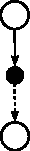
\includegraphics[width=0.5cm]{fig/lec05/Back_Up_TD.pdf}
		\caption{Back up diagram for TD(0)}
		\label{fig:Back_up_TD0}
	\end{figure}
\end{minipage}
\end{column}
\hfill
\begin{column}{0.72\textwidth}
\begin{minipage}[c]{\linewidth}
	\begin{itemize}
		\item TD as well as MC use \hl{sample updates}.
		\item Looking ahead to a sample successor state including its value and the reward along the way to compute a backed up value estimate.
	\end{itemize}
\end{minipage}
\end{column}
\end{columns}
\vspace{0.5cm}\pause
The \hl{TD error} is:
\begin{equation}
	\delta_k = r_{k+1}+\gamma \hat{v}(x_{k+1}) - \hat{v}(x_{k}).
\end{equation}
\begin{itemize}
	\item $\delta_k$ is available at time step $k+1$.
	\item Iteratively $\delta_k$ converges towards zero. 
\end{itemize}
}

%%%%%%%%%%%%%%%%%%%%%%%%%%%%%%%%%%%%%%%%%%%%%%%%%%%%%%%%%%%%%
%% TD Error and its Relation to the MC Error %%
%%%%%%%%%%%%%%%%%%%%%%%%%%%%%%%%%%%%%%%%%%%%%%%%%%%%%%%%%%%%%
\frame{\frametitle{TD Error and its Relation to the MC Error }
\onslide<1->{Let's assume that the TD(0) estimate $\hat{v}(x)$ is not changing over one episode as it would be for MC prediction: 
\begin{equation}
\begin{split}
\underbrace{g_k - \hat{v}(x_k)}_{\mbox{MC-error}} &= r_{k+1} + \gamma g_{k+1} - \hat{v}(x_k)	+\gamma  \hat{v}(x_{k+1})	-\gamma  \hat{v}(x_{k+1}),\\}
																									\onslide<2->{&=\delta_k + \gamma(g_{k+1} - \hat{v}(x_{k+1})),\\}
																									\onslide<3->{&=\delta_k + \gamma \delta_{k+1} + \gamma^2(g_{k+2} - \hat{v}(x_{k+2})),\\}
																									\onslide<4->{&=\delta_k + \gamma \delta_{k+1} + \gamma^2 \delta_{k+2} +\gamma^3(g_{k+3} - \hat{v}(x_{k+3})),\\}
																									\onslide<5->{&=\cdots ,\\
																									&=\sum_{i=k}^{T-1} \gamma^{i-k}\delta_i.}
\end{split}
\end{equation}
\onslide<5->{
\begin{itemize}
	\item MC error is the discounted sum of TD errors in this simplified case.
	\item If $\hat{v}(x)$ is updated during one episode (as expected in TD(0)), the above identity only holds approximately. 
\end{itemize}}
}

%%%%%%%%%%%%%%%%%%%%%%%%%%%%%%%%%%%%%%%%%%%%%%%%%%%%%%%%%%%%%
%% Overview of the RL methods considered so far %%
%%%%%%%%%%%%%%%%%%%%%%%%%%%%%%%%%%%%%%%%%%%%%%%%%%%%%%%%%%%%%
\frame{\frametitle{Overview of the RL Methods Considered so far}
\begin{figure}		
	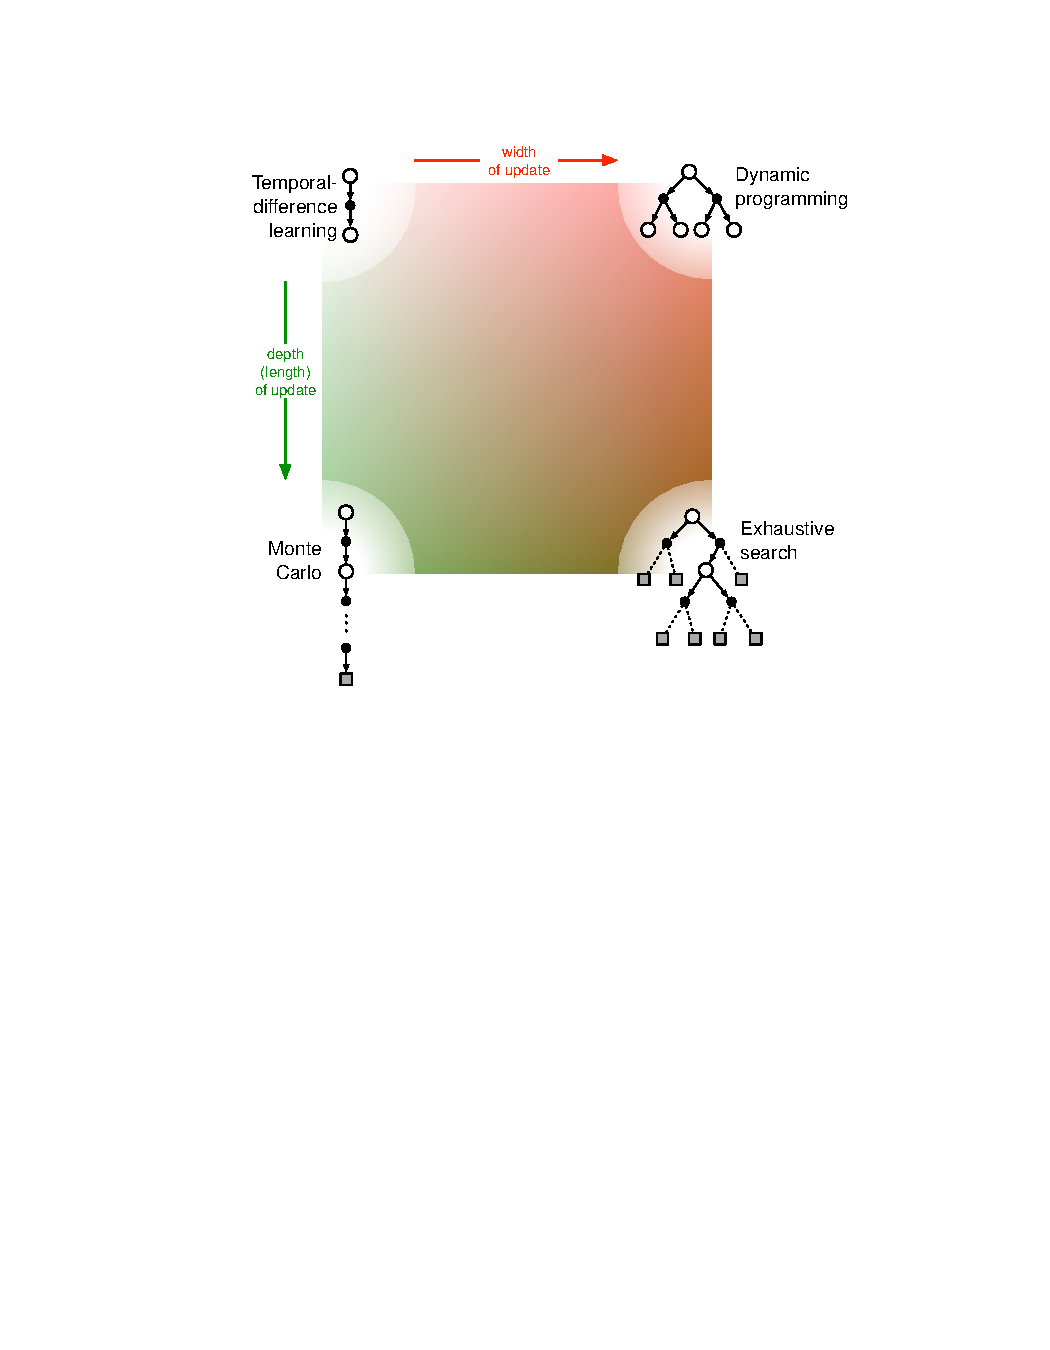
\includegraphics[width=7cm]{fig/lec05/Compare_RL_Methods_Update.pdf}
	\caption{Comparison of the RL methods considered so far with regard to the update rules (source: R. Sutton and G. Barto, Reinforcement learning: an introduction, 2018, \href{https://creativecommons.org/licenses/by-nc-nd/2.0/}{CC BY-NC-ND 2.0})}
	\label{fig:Compare_RL_Methods_Update}
\end{figure}
}

%%%%%%%%%%%%%%%%%%%%%%%%%%%%%%%%%%%%%%%%%%%%%%%%%%%%%%%%%%%%%
%% Driving Home Example (1) %%
%%%%%%%%%%%%%%%%%%%%%%%%%%%%%%%%%%%%%%%%%%%%%%%%%%%%%%%%%%%%%
\frame{\frametitle{Driving Home Example (1)}
\begin{table}
	\centering
		\begin{tabular}{l|M{2cm}|M{2cm}|M{2cm}}
			\onslide<1->{
			state & elapsed time  & predicted time to go & predicted total time\\
			\hline
			leaving office & 0 & 30 & 30\\
			}
			\onslide<2->reaching car, raining & 5 & 35 &40\\
			\onslide<3->exiting highway & 20 & 15 & 35\\
			\onslide<4->behind truck & 30 & 10 & 40\\
			\onslide<5->home street & 40 & 3 & 43\\
			\onslide<6->arrive home & 43 & 0 &43
		\end{tabular}	
	\onslide<1->\caption{Exemplary driving home journey assuming a given policy and all numbers denote minutes (source: R. Sutton and G. Barto, Reinforcement learning: an introduction, 2018, \href{https://creativecommons.org/licenses/by-nc-nd/2.0/}{CC BY-NC-ND 2.0})}
	\label{tab:driving_home_example}
\end{table}

}

%%%%%%%%%%%%%%%%%%%%%%%%%%%%%%%%%%%%%%%%%%%%%%%%%%%%%%%%%%%%%
%% Driving Home Example (2) %%
%%%%%%%%%%%%%%%%%%%%%%%%%%%%%%%%%%%%%%%%%%%%%%%%%%%%%%%%%%%%%
\frame{\frametitle{Driving Home Example (2)}
\begin{figure}		
	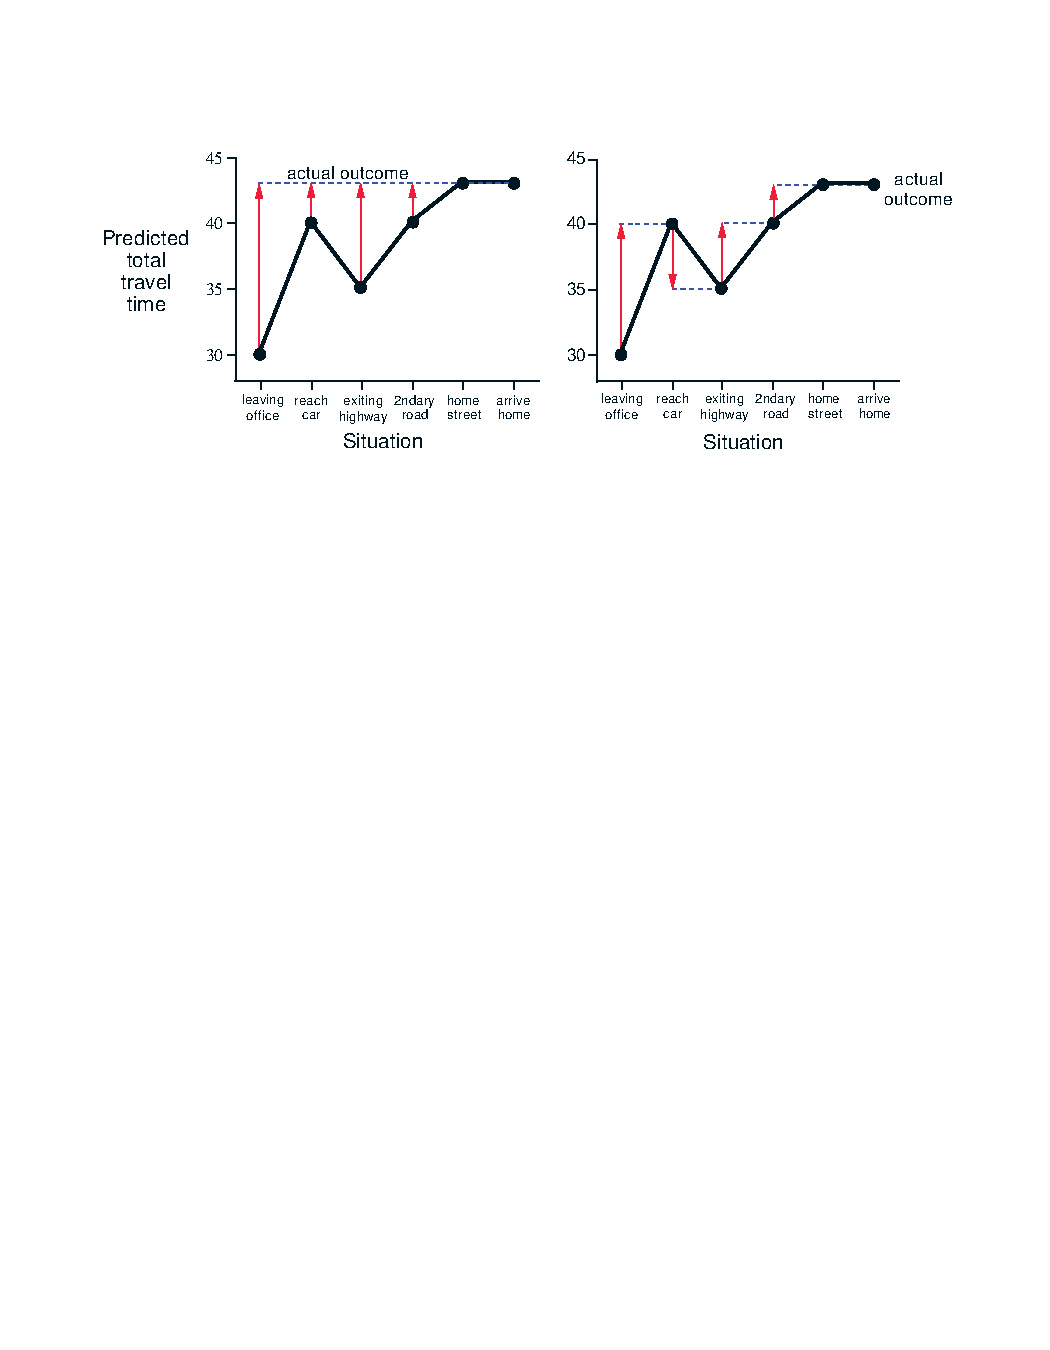
\includegraphics[width=10cm]{fig/lec05/Driving_home_example.pdf}
	\caption{Updates by MC (left) and TD (right) for $\alpha = 1$ (source: R. Sutton and G. Barto, Reinforcement learning: an introduction, 2018, \href{https://creativecommons.org/licenses/by-nc-nd/2.0/}{CC BY-NC-ND 2.0})}
	\label{fig:Driving_home_example}
\end{figure}
\begin{itemize}
	\item TD can learn before knowing the final outcome.
	\begin{itemize}
		\item TD learns after every step.
		\item MC must wait until the episode's end.
	\end{itemize}
	\item TD could learn without a final outcome.
	\begin{itemize}
		\item MC is only applicable to episodic tasks.
		\item TD can learn from incomplete sequences, i.e., in continuing tasks.
	\end{itemize}
\end{itemize}
}

%%%%%%%%%%%%%%%%%%%%%%%%%%%%%%%%%%%%%%%%%%%%%%%%%%%%%%%%%%%%%
%% TD(0) Prediction Example: Forest Tree MDP (1 )%%
%%%%%%%%%%%%%%%%%%%%%%%%%%%%%%%%%%%%%%%%%%%%%%%%%%%%%%%%%%%%%
\frame{\frametitle{TD(0) Prediction Example: Forest Tree MDP (1)}
Let's reuse the forest tree MDP example with \textit{fifty-fifty policy} and discount factor $\gamma=0.8$
plus disaster probability $\alpha=0.2$:
\vspace{0.5cm}
\begin{figure}		
	%\hspace*{-1.5cm}
	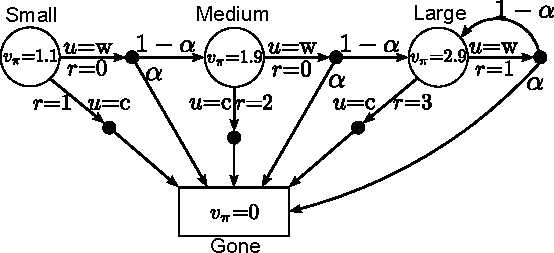
\includegraphics[width=9cm]{fig/lec04/Forest_Markov_Decision_Process_State_Value.pdf}
	\caption{Forest MDP with fifty-fifty-policy including state values}
\end{figure}
}

%%%%%%%%%%%%%%%%%%%%%%%%%%%%%%%%%%%%%%%%%%%%%%%%%%%%%%%%%%%%%
%% TD(0) Prediction Example: Forest Tree MDP(2)%%
%%%%%%%%%%%%%%%%%%%%%%%%%%%%%%%%%%%%%%%%%%%%%%%%%%%%%%%%%%%%%
\frame{\frametitle{TD(0) Prediction Example: Forest Tree MDP (2)}
\vspace{-0.5cm}
\begin{figure}		
\hspace*{-1.0cm}
	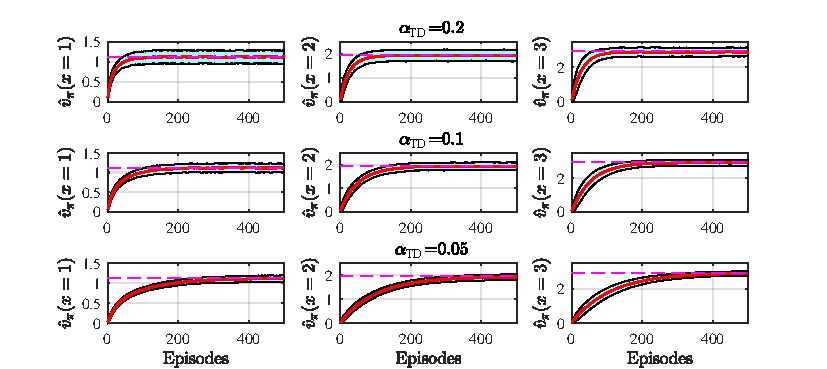
\includegraphics{fig/lec05/Forest_Tree_TD0_Prediction.pdf}
	\caption{State-value estimate of forest tree MDP using TD(0) prediction over the number of episodes being evaluated (mean and standard deviation are calculated based on 2000 independent runs)}
	\label{fig:Forest_Tree_TD0_Prediction}
\end{figure}
}

%%%%%%%%%%%%%%%%%%%%%%%%%%%%%%%%%%%%%%%%%%%%%%%%%%%%%%%%%%%%%
%% TD(0) vs. MC Prediction Example: Forest Tree MDP(1)%%
%%%%%%%%%%%%%%%%%%%%%%%%%%%%%%%%%%%%%%%%%%%%%%%%%%%%%%%%%%%%%
\frame{\frametitle{TD(0) vs. MC Prediction Example: Forest Tree MDP (1)}
\vspace{-0.25cm}
\begin{figure}		
\hspace*{-0.5cm}
	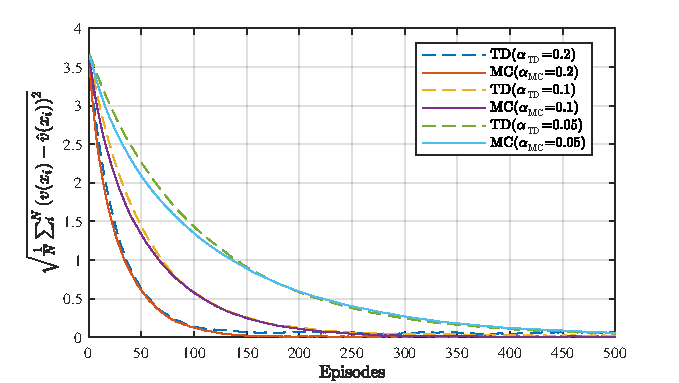
\includegraphics{fig/lec05/Forest_Tree_TD0_MC_RMS_Prediction_Zero_Init_500_eps.pdf}
	\caption{Averaged mean of state-value estimates of forest tree MDP using TD(0) and MC over 1000 independent runs with $\hat{v}_0(x)=0\,\forall x\in\mathcal{X}$}
	\label{fig:Forest_Tree_TD0_MC_RMS_Prediction_Zero_Init_500_eps}
\end{figure}
}

%%%%%%%%%%%%%%%%%%%%%%%%%%%%%%%%%%%%%%%%%%%%%%%%%%%%%%%%%%%%%
%% TD(0) Prediction Example: Forest Tree MDP(2)%%
%%%%%%%%%%%%%%%%%%%%%%%%%%%%%%%%%%%%%%%%%%%%%%%%%%%%%%%%%%%%%
\frame{\frametitle{TD(0) vs. MC Prediction Example: Forest Tree MDP (2)}
\vspace{-0.25cm}
\begin{figure}		
\hspace*{-0.5cm}
	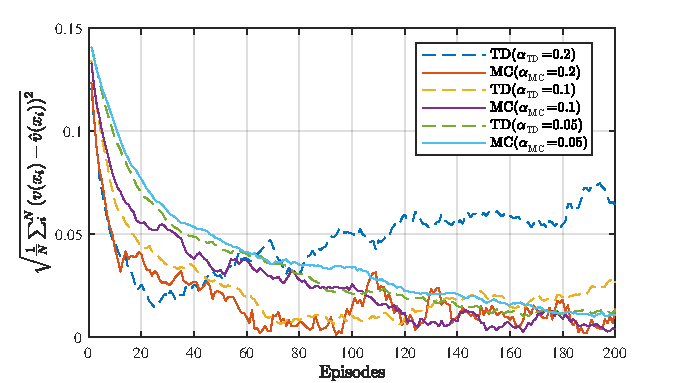
\includegraphics{fig/lec05/Forest_Tree_TD0_MC_RMS_Prediction_Good_Init_200_eps.pdf}
	\caption{Averaged mean of state-value estimates of forest tree MDP using TD(0) and MC over 1000 independent runs with \hl{$\hat{v}_0(x)\approx v(x) \,\forall x\in\mathcal{X}$}}
	\label{fig:Forest_Tree_TD0_MC_RMS_Prediction_Good_Init_200_eps}
\end{figure}
}

%%%%%%%%%%%%%%%%%%%%%%%%%%%%%%%%%%%%%%%%%%%%%%%%%%%%%%%%%%%%%
%% Convergence of TD(0)%%
%%%%%%%%%%%%%%%%%%%%%%%%%%%%%%%%%%%%%%%%%%%%%%%%%%%%%%%%%%%%%
\frame{\frametitle{Convergence of TD(0)}
\begin{theo}{Convergence of TD(0)}{converge_TD_zero}
Given a finite MDP and a fixed policy $\pi$ the state-value estimate of TD(0) converges to the true $v_\pi$
\begin{itemize}
	\item in the mean for a constant but sufficiently small step-size $\alpha$ and
	\item with probability 1 if the step-size holds the condition
	\begin{equation}
		\sum_{k=1}^{\infty}  \alpha_k = \infty \quad \mbox{and} \quad \sum_{k=1}^{\infty}  \alpha_k^2 < \infty .
		\label{eq:stoch_approx_condition}
	\end{equation}
\end{itemize}
Above $k$ is the sample index (i.e., how often the TD update was applied). 
\end{theo}\pause
\begin{itemize}
	\item In particular, $\alpha_k=\frac{1}{k}$ meets the condition \eqref{eq:stoch_approx_condition}.\pause
	\item Often TD(0) converges faster than MC, but there is no guarantee (see examples above and in Barto/Sutton book).\pause
	\item TD(0) can be more sensitive to bad initializations $\hat{v}_0(x)$ compared to MC.
\end{itemize}
}

%%%%%%%%%%%%%%%%%%%%%%%%%%%%%%%%%%%%%%%%%%%%%%%%%%%%%%%%%%%%%
%% Batch Training%%
%%%%%%%%%%%%%%%%%%%%%%%%%%%%%%%%%%%%%%%%%%%%%%%%%%%%%%%%%%%%%
\frame{\frametitle{Batch Training}
\begin{itemize}
	\item If experience $\rightarrow\infty$ both MC and TD converge $\hat{v}(x)\rightarrow v(x)$.
	\item But how to handle limited experience, i.e., a finite set of episodes
	\begin{align*}
		&x_{1,1}, u_{1,1} , r_{2,1}, \ldots, x_{T_1,1},\\
		&x_{1,2}, u_{1,2} , r_{2,2}, \ldots, x_{T_2,2},\\
		&\hspace{2cm}\vdots\\
		&x_{1,j}, u_{1,j} , r_{2,j}, \ldots, x_{T_j,j},\\
		&\hspace{2cm}\vdots\\
		&x_{1,J}, u_{1,J} , r_{2,J}, \ldots, x_{T_J,J}.
	\end{align*}
\end{itemize}\pause
\begin{block}{Batch training}
\begin{itemize}
	\item Process all available episodes $j\in\left[1,J\right]$ repeatedly to MC and TD.
	\item If the step size $\alpha$ is sufficiently small both will converge to certain steady-state values. 
\end{itemize}
\end{block}
}

%%%%%%%%%%%%%%%%%%%%%%%%%%%%%%%%%%%%%%%%%%%%%%%%%%%%%%%%%%%%%
%% Batch Training: AB-Example (1) %%
%%%%%%%%%%%%%%%%%%%%%%%%%%%%%%%%%%%%%%%%%%%%%%%%%%%%%%%%%%%%%
\frame{\frametitle{Batch Training: AB-Example (1)}
\begin{columns}[t,onlytextwidth]
\begin{column}{0.58\textwidth}
\begin{minipage}[c]{\linewidth}
	\begin{figure}
		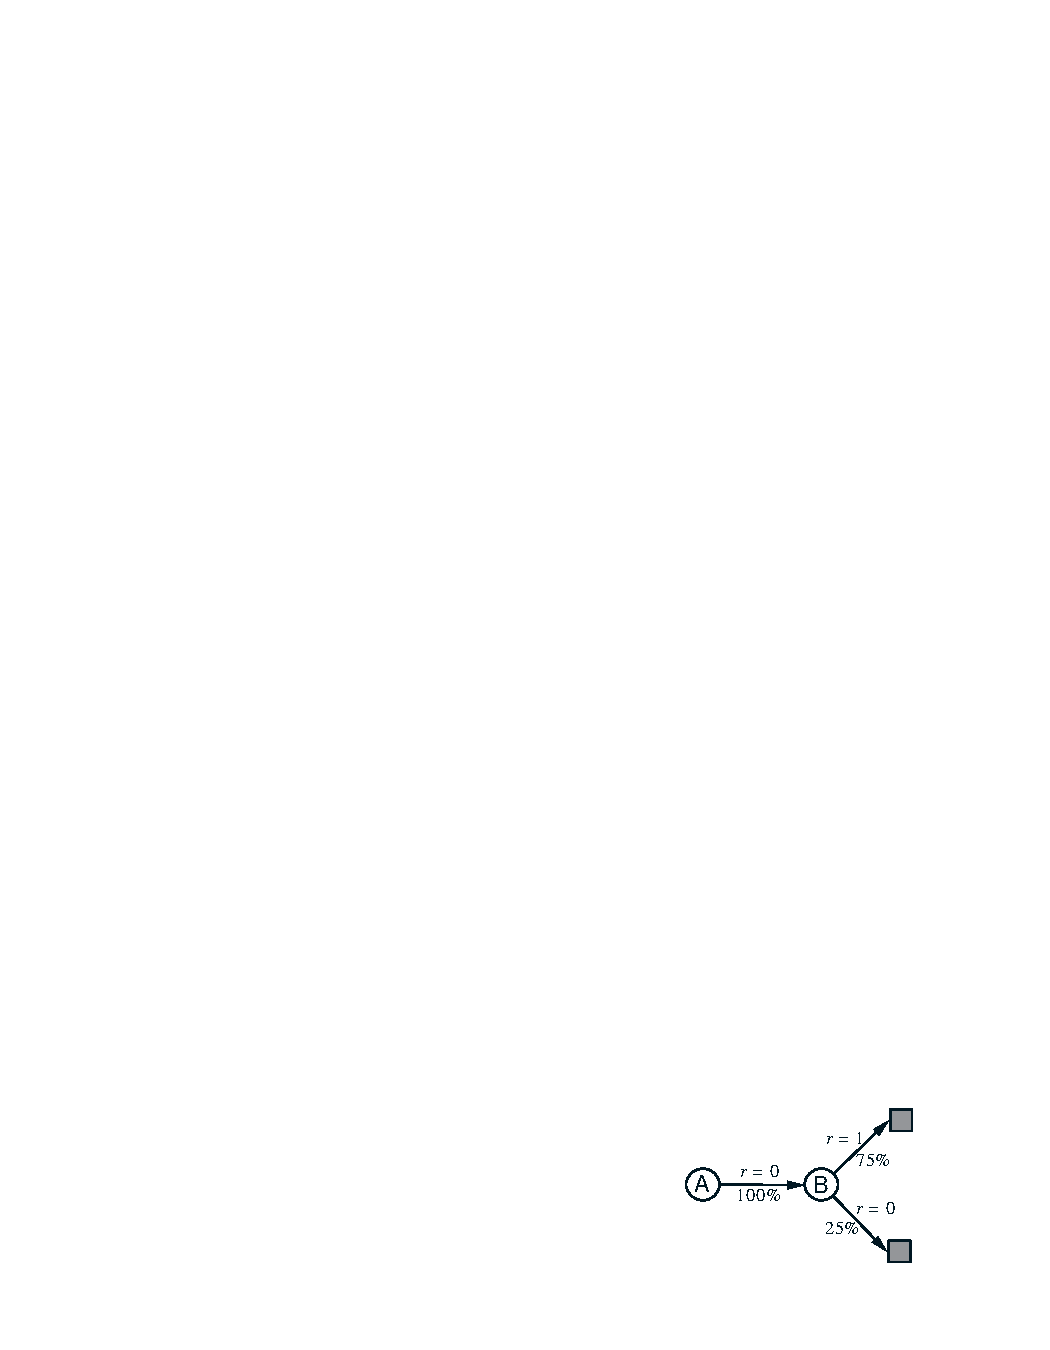
\includegraphics[width=4.5cm]{fig/lec05/Batch_AB_Example.pdf}
		\caption{Example environment (source: R. Sutton and G. Barto, Reinforcement learning: an introduction, 2018, \href{https://creativecommons.org/licenses/by-nc-nd/2.0/}{CC BY-NC-ND 2.0})}
		\label{fig:Batch_AB_Example}
	\end{figure}
\end{minipage}
\end{column}
\hfill
\begin{column}{0.40\textwidth}
\begin{minipage}[c]{\linewidth}
	\begin{itemize}
		\item Only two states: A, B
		\item No discounting
		\item 8 episodes of experience available (see \tabref{tab:state_reward_AB_example})
		\item What is $\hat{v}(A)$ and $\hat{v}(B)$ using batch training TD(0) and MC?
	\end{itemize}
\end{minipage}
\end{column}
\end{columns}
\vspace{0.25cm}
\begin{table}
	\centering
		\begin{tabular}{M{2cm}|M{2cm}}
			A, 0, B, 0 & B,1\\
			\hline
			B,1 & B,1\\
			\hline
			B,1	& B,1\\
			\hline
			B,1	& B,0
		\end{tabular}	
	\caption{Example state-reward sequences for \figref{fig:Batch_AB_Example}}
	\label{tab:state_reward_AB_example}
\end{table}
}

%%%%%%%%%%%%%%%%%%%%%%%%%%%%%%%%%%%%%%%%%%%%%%%%%%%%%%%%%%%%%
%% Batch Training: AB-Example (2) %%
%%%%%%%%%%%%%%%%%%%%%%%%%%%%%%%%%%%%%%%%%%%%%%%%%%%%%%%%%%%%%
\frame{\frametitle{Batch Training: AB-Example (2)}
First, recap MC and TD(0) update rules:
\begin{align*}
	\mbox{MC}: \quad &\hat{v}(x_k) \leftarrow \hat{v}(x_k) + \alpha\left[g_k - \hat{v}(x_k)\right],\\
	\mbox{TD}:	\quad&\hat{v}(x_k) \leftarrow \hat{v}(x_k) + \alpha\left[r_{k+1}+\gamma\hat{v}(x_{k+1}) - \hat{v}(x_k)\right] .
\end{align*}\pause
Then, in steady state one receives:  
\begin{align*}
	\mbox{MC}: \quad &0=\alpha\left[g_k - \hat{v}(x_k)\right]=g_k - \hat{v}(x_k),\\
	\mbox{TD}:	\quad&0=\alpha\left[r_{k+1}+\gamma\hat{v}(x_{k+1}) - \hat{v}(x_k)\right] =r_{k+1}+\gamma\hat{v}(x_{k+1}) - \hat{v}(x_k).
\end{align*}\pause
Considering a batch learning sweep over $j=1,\ldots,J$ episodes:
\begin{align*}
	\mbox{MC}: \quad &0=\sum_{j=1}^J g_{k,j} - \hat{v}(x_{k,j}),\\
	\mbox{TD}:	\quad&0=\sum_{j=1}^J r_{k+1,j}+\gamma\hat{v}(x_{k+1,j}) - \hat{v}(x_{k,j}).
\end{align*}
}

%%%%%%%%%%%%%%%%%%%%%%%%%%%%%%%%%%%%%%%%%%%%%%%%%%%%%%%%%%%%%
%% Batch Training: AB-Example (3) %%
%%%%%%%%%%%%%%%%%%%%%%%%%%%%%%%%%%%%%%%%%%%%%%%%%%%%%%%%%%%%%
\frame{\frametitle{Batch Training: AB-Example (3)}
Apply the previous equations first to state B. Since B is a terminal state, $\hat{v}(x_{k+1})=0$ and $g_{k,j}= r_{k+1,j}$ apply, i.e., the MC and TD updates are identical for B:
\begin{alignat*}{3}
	\mbox{MC}|_{x=\mbox{B}}: \quad &0=\sum_{j=1}^J g_{k,j} - \hat{v}(x_{k,j})\quad &&\Leftrightarrow \quad &&\hat{v}(\mbox{B})=\frac{1}{J}\sum_{j=1}^J g_{k,j},\\
	\mbox{TD}|_{x=\mbox{B}}:	\quad&0=\sum_{j=1}^J r_{k+1,j}- \hat{v}(x_{k,j})\quad &&\Leftrightarrow \quad &&\hat{v}(\mbox{B})=\frac{1}{J}\sum_{j=1}^J g_{k,j}.
\end{alignat*}\pause
This is the average return of the available episodes from \tabref{tab:state_reward_AB_example} , i.e., $6\times 1$ and $2\times 0$:
\begin{equation}
	\hat{v}(\mbox{B})|_{\mbox{MC}}=\hat{v}(\mbox{B})|_{\mbox{TD}}=\frac{6}{8}=0.75\, .
\end{equation}
}

%%%%%%%%%%%%%%%%%%%%%%%%%%%%%%%%%%%%%%%%%%%%%%%%%%%%%%%%%%%%%
%% Batch Training: AB-Example (4) %%
%%%%%%%%%%%%%%%%%%%%%%%%%%%%%%%%%%%%%%%%%%%%%%%%%%%%%%%%%%%%%
\frame{\frametitle{Batch Training: AB-Example (4)}
Now consider state A assuming the steady state of batch learning process:
\begin{itemize}
	\item The instantaneous reward is always $r=0$.
	\item The TD bootstrap estimate of B is $\hat{v}(x_{k+1,j})=\hat{v}(B)=\frac{3}{4}$.
\end{itemize}\pause
\begin{align*}
	\mbox{MC}: \quad &0=\sum_{j=1}^J g_{k,j} - \hat{v}(x_{k,j})=\sum_{j=1}^J g_{k,j} - \hat{v}(A),\\
	\mbox{TD}:	\quad&0=\sum_{j=1}^J r_{k+1,j}+\gamma\hat{v}(x_{k+1,j}) - \hat{v}(x_{k,j})=\sum_{j=1}^J \gamma\hat{v}(B) - \hat{v}(A).
\end{align*}\pause
Looking at \tabref{tab:state_reward_AB_example} there is only one episode visiting state A, where the sample return is $g_{k,j}=0$. Hence, it follows: 
\begin{equation*}
	\hat{v}(\mbox{A})|_{\mbox{MC}} =0, \quad \hat{v}(\mbox{A})|_{\mbox{TD}} =\gamma\hat{v}(B)=\frac{3}{4}.
\end{equation*}
Where does this mismatch between the MC and TD estimates come from?
}

%%%%%%%%%%%%%%%%%%%%%%%%%%%%%%%%%%%%%%%%%%%%%%%%%%%%%%%%%%%%%
%% Certainty Equivalence %%
%%%%%%%%%%%%%%%%%%%%%%%%%%%%%%%%%%%%%%%%%%%%%%%%%%%%%%%%%%%%%
\frame{\frametitle{Certainty Equivalence}
\begin{itemize}
	\item MC batch learning converges to the \hl{least squares fit} of the sampled returns:
	\begin{equation}
		\sum_{j=1}^{J}\sum_{k=1}^{T_j} \left(g_{k,j}- \hat{v}(x_{k,j})\right)^2 .
	\end{equation}\pause\vspace{-0.25cm}
	\item TD batch learning converges to the \hl{maximum likelihood estimate} such that $\left\langle\mathcal{X}, \mathcal{U}, \hat{\mathcal{P}}, \hat{\mathcal{R}}, \gamma \right\rangle$ explains the data with highest probability:
	\begin{equation}
		\begin{split}
		\hat{p}_{xx'}^u&=\frac{1}{n(x,u)}\sum_{j=1}^{J}\sum_{k=1}^{T_j} 1(X_{k+1}=x'|X_{k}=x, U_k=u),\\
		\hat{\mathcal{R}}_{x}^u&=\frac{1}{n(x,u)}\sum_{j=1}^{J}\sum_{k=1}^{T_j} 1(X_{k}=x|U_k=u) r_{k+1,j}.
	\end{split}
	\end{equation}
	\item Here, TD assumes a MDP problem structure and is absolutely certain that its model estimate describes the real world perfectly (so-called \hl{certainty equivalence}).
\end{itemize}
}

%%%%%%%%%%%%%%%%%%%%%%%%%%%%%%%%%%%%%%%%%%%%%%%%%%%%%%%%%%%%%%%%%%
\section{Temporal-Difference On-Policy Control: Sarsa} 
%%%%%%%%%%%%%%%%%%%%%%%%%%%%%%%%%%%%%%%%%%%%%%%%%%%%%%%%%%%%%%%%%%
\begin{frame}
\frametitle{Table of Contents}
\tableofcontents[currentsection]
\end{frame}

%%%%%%%%%%%%%%%%%%%%%%%%%%%%%%%%%%%%%%%%%%%%%%%%%%%%%%%%%%%%%
%% Applying Generalized Policy Iteration (GPI) to MC Control %%
%%%%%%%%%%%%%%%%%%%%%%%%%%%%%%%%%%%%%%%%%%%%%%%%%%%%%%%%%%%%%
\frame{\frametitle{Applying Generalized Policy Iteration (GPI) to TD Control}
GPI concept is directly applied to the TD framework using action values:
\begin{equation}
	\pi_0 \rightarrow \hat{q}_{\pi_0} \rightarrow \pi_1 \rightarrow \hat{q}_{\pi_1} \rightarrow \cdots \pi^* \rightarrow \hat{q}_{\pi^*} \, .
\end{equation}\pause
\begin{block}{One-step TD / TD(0) action-value update (Sarsa)}
	The TD(0) action-value update is:
		\begin{equation}
		\hat{q}(x_k, u_k) \leftarrow \hat{q}(x_k, u_k) + \alpha\left[r_{k+1}+\gamma\hat{q}(x_{k+1}, u_{k+1}) - \hat{q}(x_k, u_k)\right] .
		\label{eq:TD_zero_update_action_value}
		\end{equation}
		\hl{Sarsa}: \hl{s}tate, \hl{a}ction, \hl{r}eward, (next) \hl{s}tate, (next) \hl{a}ction evaluation
	\end{block}\pause
\begin{itemize}
	\item In contrast to MC: continuous online updates of policy evaluation and improvement.\pause
	\item On-policy approach requires exploration, e.g., by an $\varepsilon$-greedy policy:
	\begin{equation}
		\pi_i(u|x)\leftarrow\begin{cases}1-\varepsilon+\varepsilon/|\mathcal{U}|, \quad u=\tilde{u},\\ \varepsilon/|\mathcal{U}|, \quad u\neq\tilde{u}.\end{cases}
	\end{equation}
\end{itemize}
}

%%%%%%%%%%%%%%%%%%%%%%%%%%%%%%%%%%%%%%%%%%%%%%%%%%%%%%%%%%%%%
%% TD-Based On-Policy Control (Sarsa) %%
%%%%%%%%%%%%%%%%%%%%%%%%%%%%%%%%%%%%%%%%%%%%%%%%%%%%%%%%%%%%%
\frame{\frametitle{TD-Based On-Policy Control (Sarsa)}
\vspace{-0.2cm}
\setlength{\algomargin}{0.5em}
\begin{algorithm}[H]
\footnotesize
\SetKwInput{Input}{input} 
\SetKwInput{Output}{output}
\SetKwInput{Init}{init}
\SetKwInput{Param}{parameter}
\Param{$\varepsilon\in\left\{\mathbb{R}|0<\varepsilon<<1\right\}, \quad \alpha\in\left\{\mathbb{R}|0<\alpha<1\right\}$}
\Init{$\hat{q}(x,u)$ arbitrarily (except terminal states) $\forall \, \left\{x\in\mathcal{X}, u\in\mathcal{U}\right\}$}
\For{$j=1,2,\ldots$ episodes}{
	Initialize $x_0$\;
	Choose $u_0$ from $x_0$ using a soft policy (e.g., $\varepsilon$-greedy) derived from $\hat{q}(x,u)$\;
	$k \leftarrow 0$\;
	\Repeat{$x_k$ is terminal}{
				Take action $u_k$, observe $r_{k+1}$ and $x_{k+1}$\;
				Choose $u_{k+1}$ from $x_{k+1}$ using a soft policy derived from $\hat{q}(x,u)$\;
				$\hat{q}(x_k, u_k) \leftarrow \hat{q}(x_k, u_k) + \alpha\left[r_{k+1}+\gamma\hat{q}(x_{k+1}, u_{k+1}) - \hat{q}(x_k, u_k)\right]$\;
				$k \leftarrow k+1$\;
	}
}
\caption{TD-based on-policy control (Sarsa)}
\label{algo:Sarsa}
\end{algorithm}
Convergence properties are comparable to MC-based on-policy control:
\begin{itemize}
	\item Policy improvement theorem \theoref{theo:policy_improv_eps_greedy} holds.
	\item Greedy in the limit with infinite exploration (GLIE) from \defref{defi:GLIE} and step-size requirements in \theoref{theo:converge_TD_zero} apply. 
\end{itemize}
}

%%%%%%%%%%%%%%%%%%%%%%%%%%%%%%%%%%%%%%%%%%%%%%%%%%%%%%%%%%%%%
%% Sarsa Example: Windy Gridworld %%
\frame{\frametitle{Example: Sarsa with Windy Gridworld}
\begin{columns}[c,onlytextwidth]
\begin{column}{0.58\textwidth}
\begin{minipage}[t]{\linewidth}
	\begin{figure}
		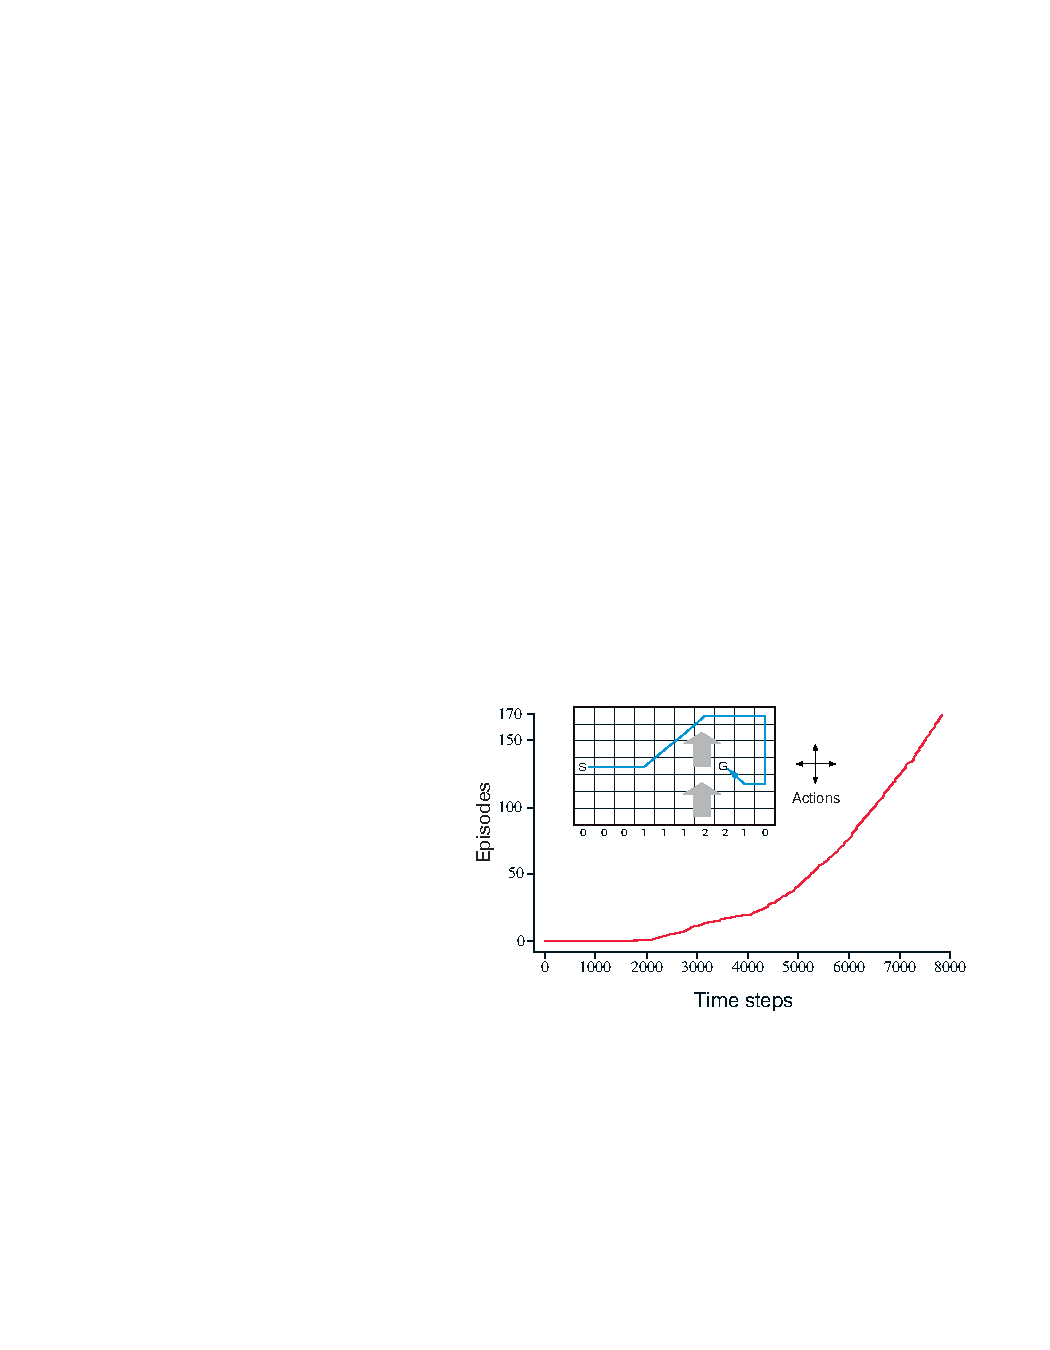
\includegraphics[width=7cm]{fig/lec05/Windy_Gridworld.pdf}
		\caption{Windy gridworld environment (source: R. Sutton and G. Barto, Reinforcement learning: an introduction, 2018, \href{https://creativecommons.org/licenses/by-nc-nd/2.0/}{CC BY-NC-ND 2.0})}
		\label{fig:Windy_Gridworld}
	\end{figure}
\end{minipage}
\end{column}
\hfill
\begin{column}{0.40\textwidth}
\begin{minipage}[t]{\linewidth}
	\begin{itemize}
		\item $r=-1$ per time step
		\item No discounting
		\item South-north wind according to value below each column
		\item $\varepsilon=0.1$
		\item $\alpha=0.5$
		\item Initial $\hat{q}(x,u)=0$ 
	\end{itemize}
	\vspace{1cm}\pause
	\begin{itemize}
		\item What could be a possible issue when applying MC control?
	\end{itemize}
\end{minipage}
\end{column}
\end{columns}
}

%%%%%%%%%%%%%%%%%%%%%%%%%%%%%%%%%%%%%%%%%%%%%%%%%%%%%%%%%%%%%
%% Sarsa Example: Forest Tree MDP (1)%%
%%%%%%%%%%%%%%%%%%%%%%%%%%%%%%%%%%%%%%%%%%%%%%%%%%%%%%%%%%%%%
\frame{\frametitle{Sarsa Example: Forest Tree MDP (1)}

\begin{figure}		
	\hspace*{-1.0cm}
	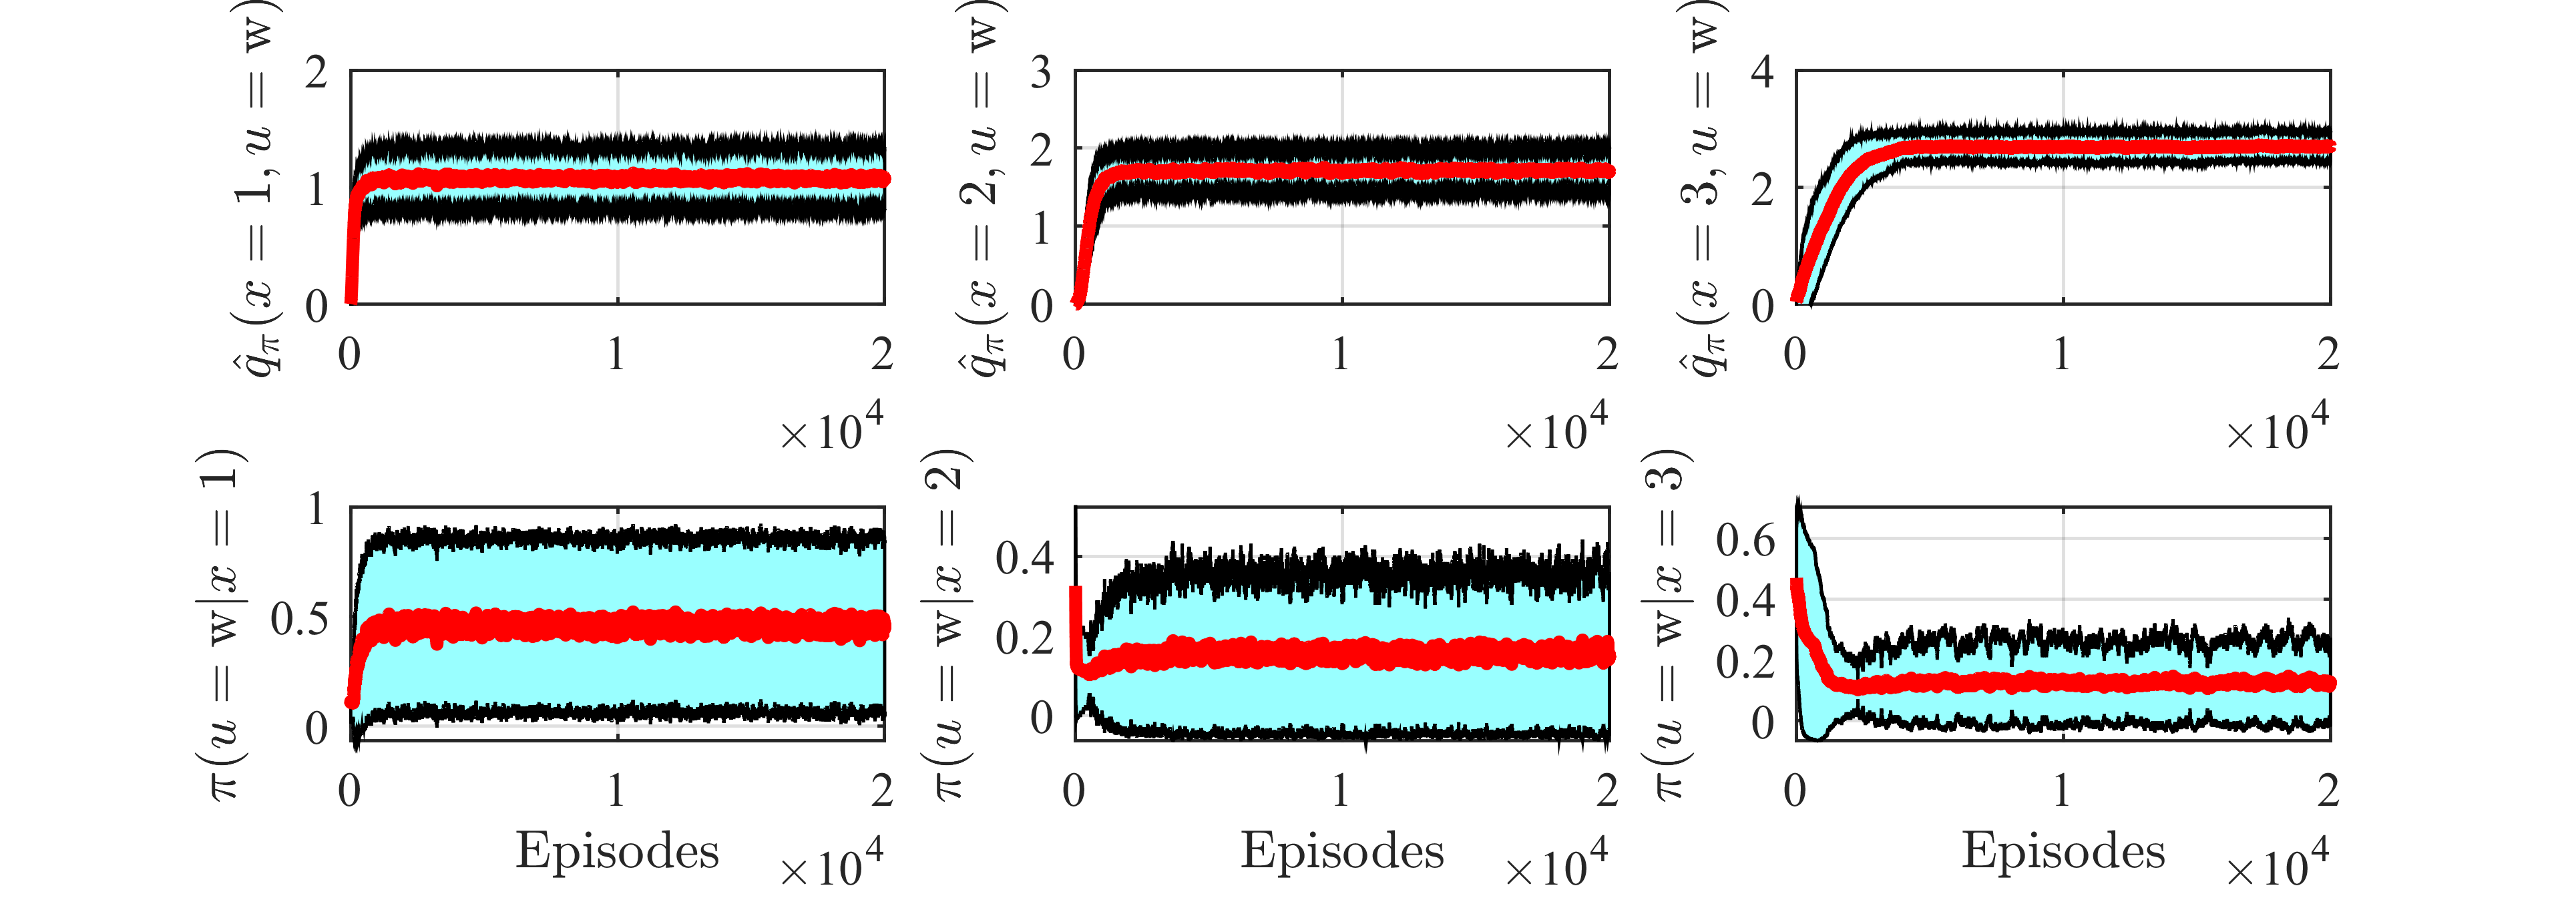
\includegraphics[width=14cm]{fig/lec05/Forest_Tree_Sarsa_alpha_0.2.png}
	\caption{Sarsa-based control with \hl{$\alpha_{Sarsa}=0.2$} and $\varepsilon$-greedy policy with $\varepsilon=0.2$ of forest tree MDP over the number of episodes being evaluated (mean and standard deviation are calculated based on 2000 independent runs)}
	\label{fig:Sarsa_forest_tree_02}
\end{figure}
}

%%%%%%%%%%%%%%%%%%%%%%%%%%%%%%%%%%%%%%%%%%%%%%%%%%%%%%%%%%%%%
%% Sarsa Example: Forest Tree MDP (2)%%
%%%%%%%%%%%%%%%%%%%%%%%%%%%%%%%%%%%%%%%%%%%%%%%%%%%%%%%%%%%%%
\frame{\frametitle{Sarsa Example: Forest Tree MDP (2)}

\begin{figure}		
	\hspace*{-1.0cm}
	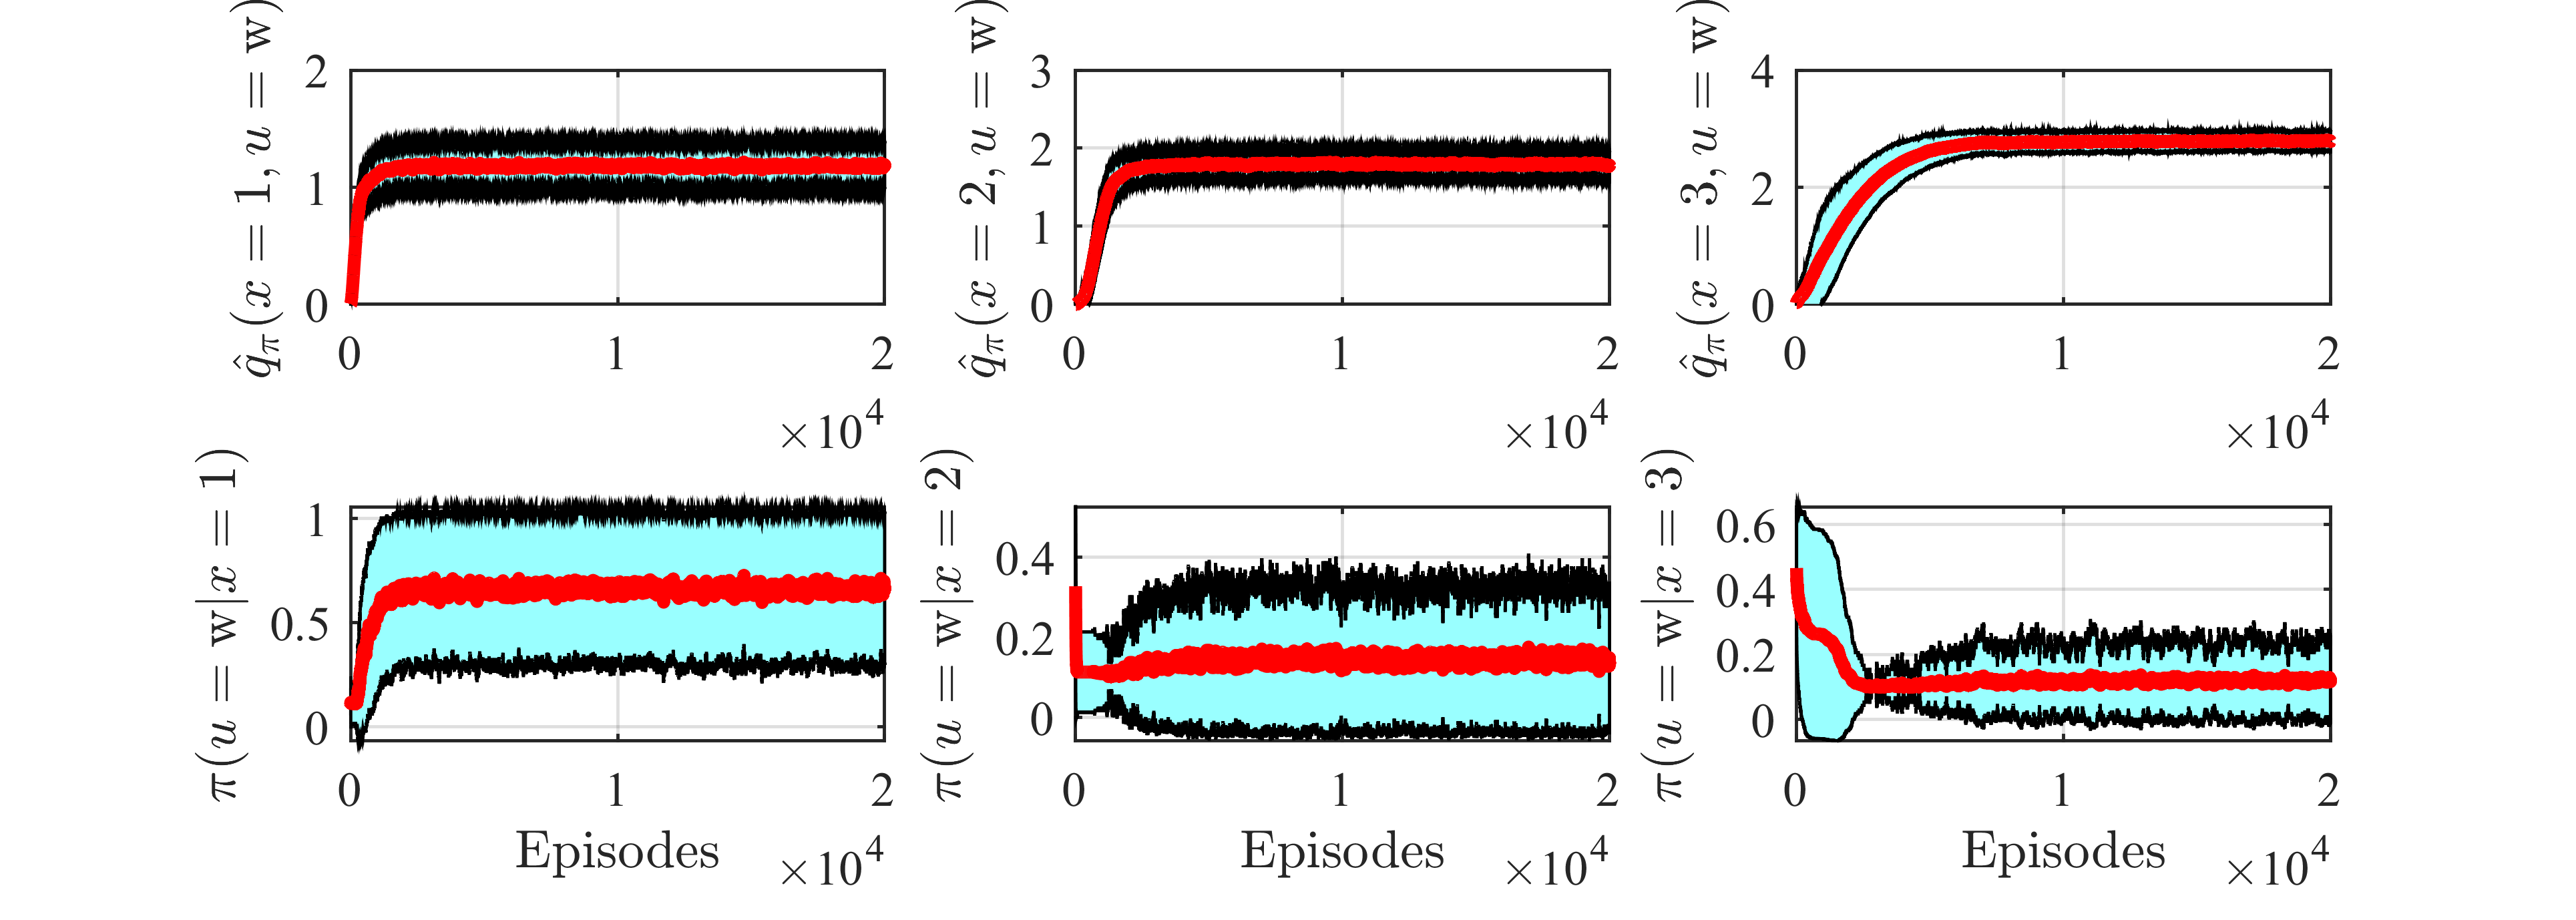
\includegraphics[width=14cm]{fig/lec05/Forest_Tree_Sarsa_alpha_0.1.png}
	\caption{Sarsa-based control with \hl{$\alpha_{Sarsa}=0.1$} and $\varepsilon$-greedy policy with $\varepsilon=0.2$ of forest tree MDP over the number of episodes being evaluated (mean and standard deviation are calculated based on 2000 independent runs)}
	\label{fig:Sarsa_forest_tree_01}
\end{figure}
}

%%%%%%%%%%%%%%%%%%%%%%%%%%%%%%%%%%%%%%%%%%%%%%%%%%%%%%%%%%%%%
%% Sarsa Example: Forest Tree MDP (3)%%
%%%%%%%%%%%%%%%%%%%%%%%%%%%%%%%%%%%%%%%%%%%%%%%%%%%%%%%%%%%%%
\frame{\frametitle{Sarsa Example: Forest Tree MDP (3)}

\begin{figure}		
	\hspace*{-1.0cm}
	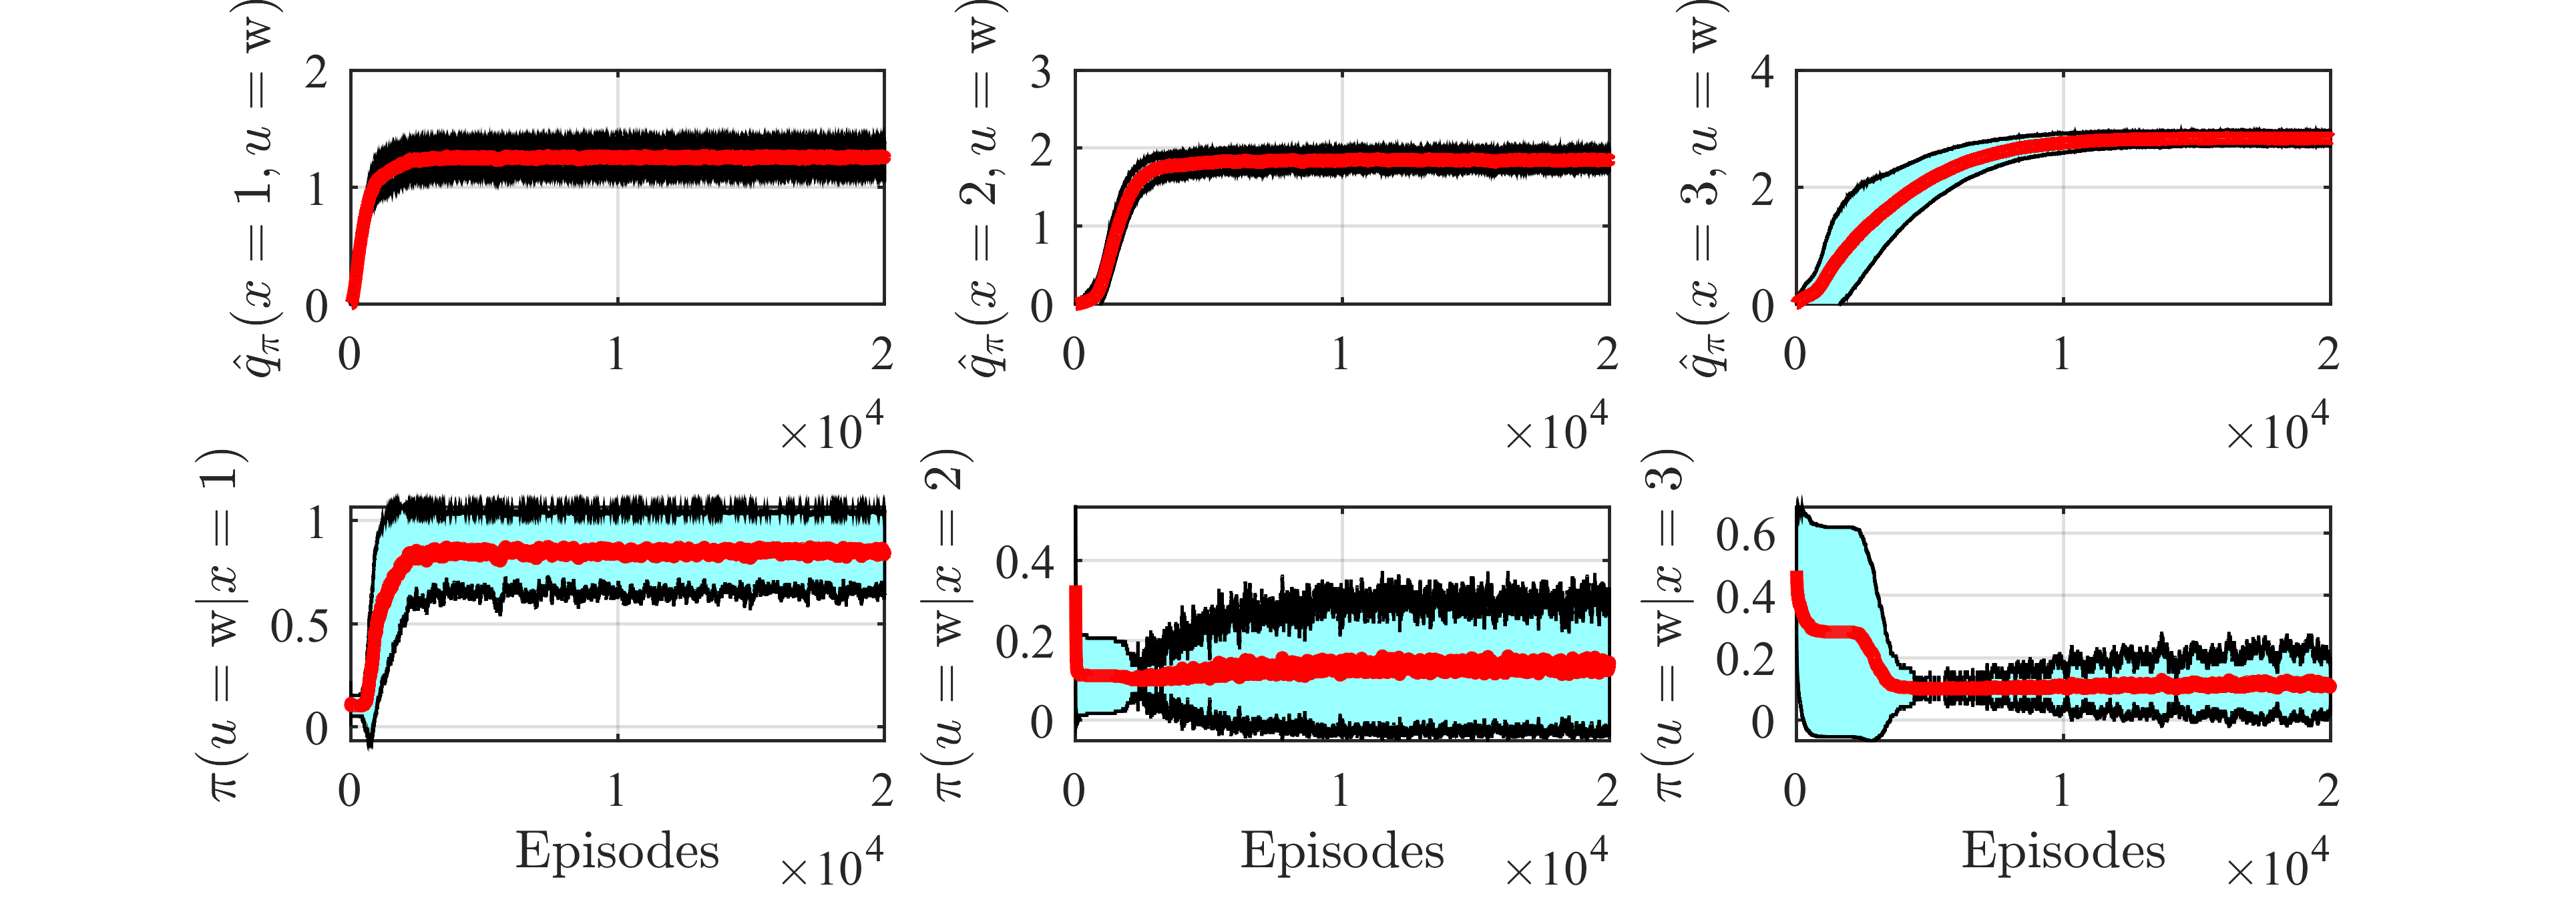
\includegraphics[width=14cm]{fig/lec05/Forest_Tree_Sarsa_alpha_0.05.png}
	\caption{Sarsa-based control with \hl{$\alpha_{Sarsa}=0.05$} and $\varepsilon$-greedy policy with $\varepsilon=0.2$ of forest tree MDP over the number of episodes being evaluated (mean and standard deviation are calculated based on 2000 independent runs)}
	\label{fig:Sarsa_forest_tree_005}
\end{figure}
}

%%%%%%%%%%%%%%%%%%%%%%%%%%%%%%%%%%%%%%%%%%%%%%%%%%%%%%%%%%%%%
%% Sarsa Example: Forest Tree MDP (4)%%
%%%%%%%%%%%%%%%%%%%%%%%%%%%%%%%%%%%%%%%%%%%%%%%%%%%%%%%%%%%%%
\frame{\frametitle{Sarsa Example: Forest Tree MDP (4)}

\begin{figure}		
	\hspace*{-1.0cm}
	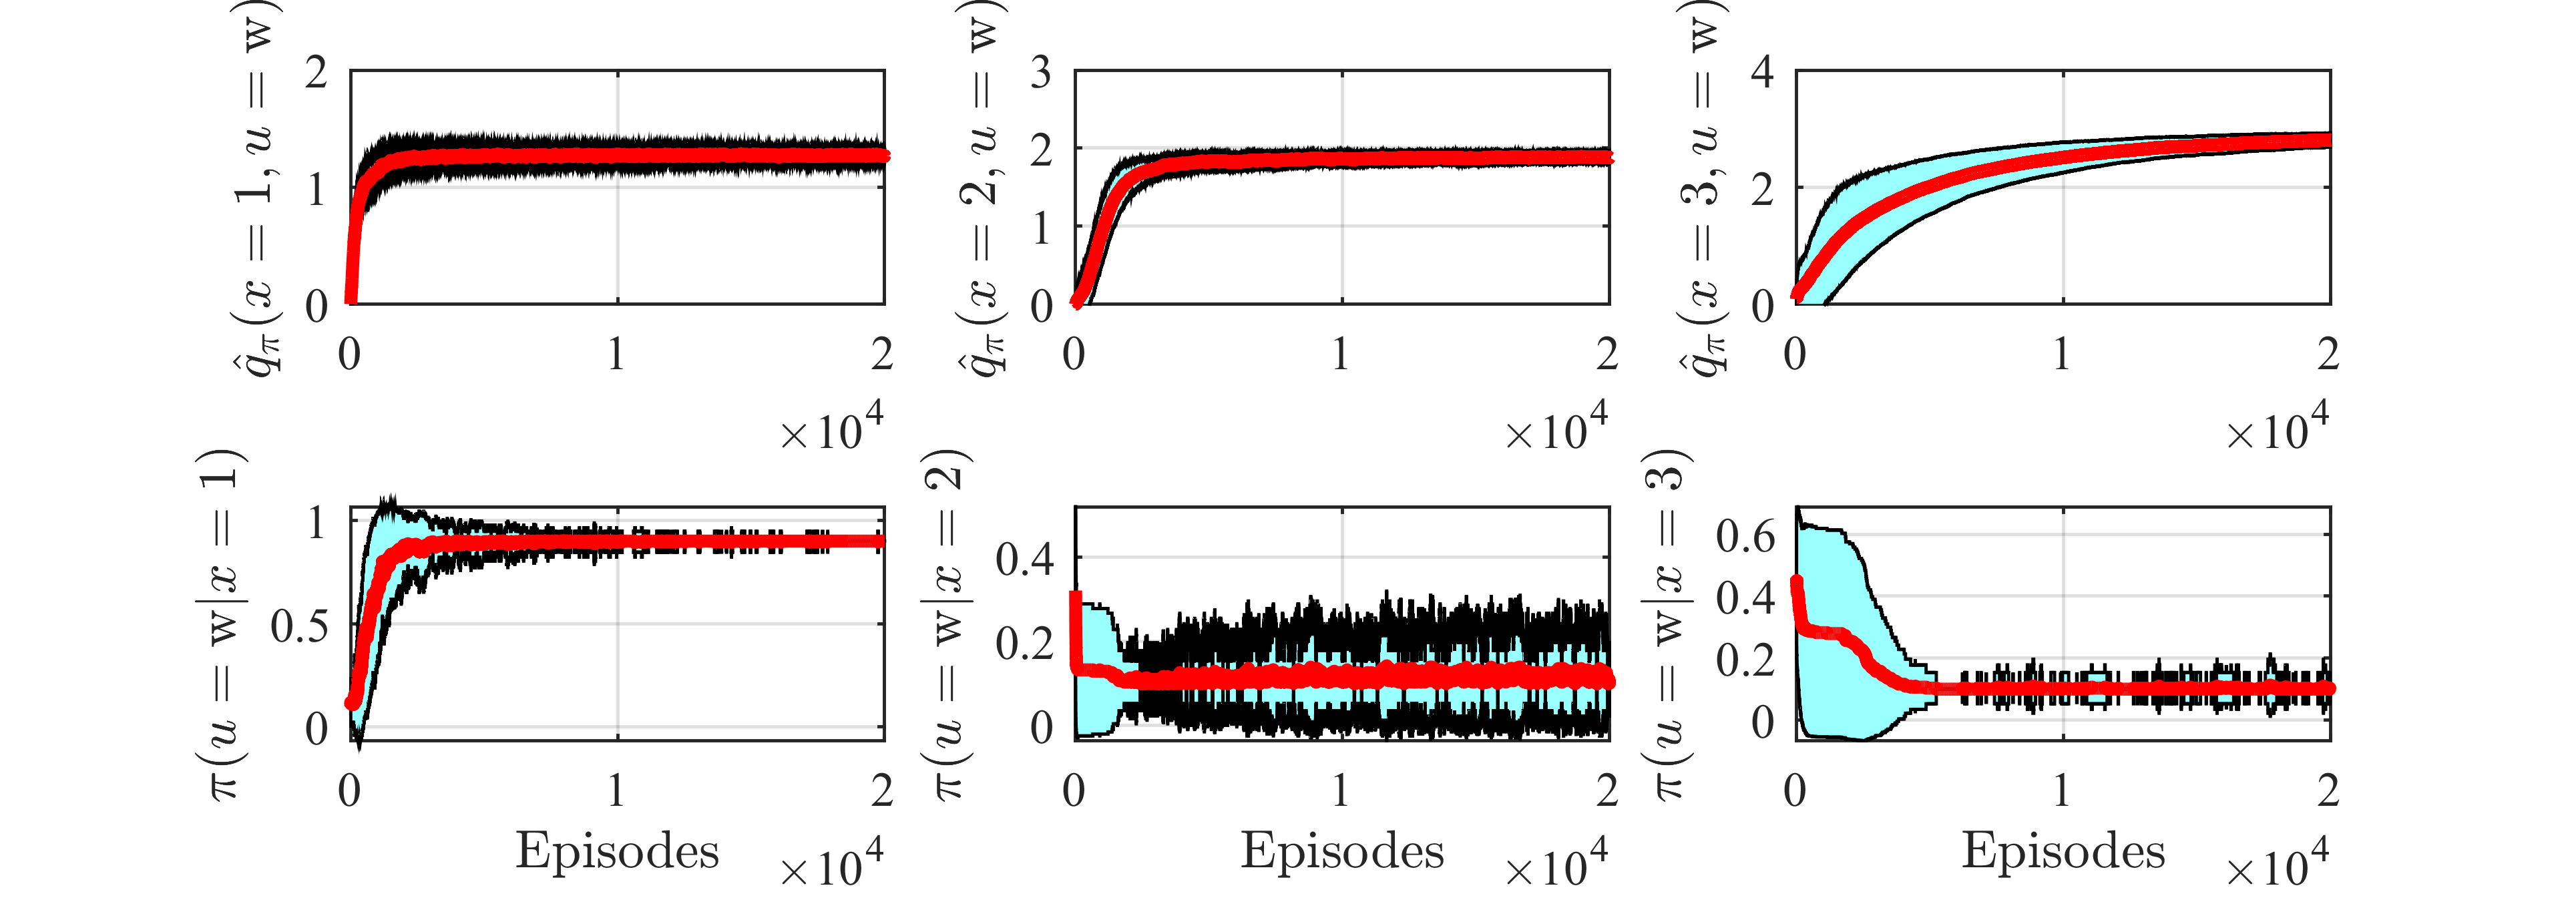
\includegraphics[width=14cm]{fig/lec05/Forest_Tree_Sarsa_alpha_adapt}
	\caption{Sarsa-based control with \hl{adaptive $\alpha_{Sarsa}=\frac{1}{\sqrt{j}}$} ($j=$episode) and $\varepsilon$-greedy policy with $\varepsilon=0.2$ of forest tree MDP over the number of episodes being evaluated (mean and standard deviation are calculated based on 2000 independent runs)}
	\label{Forest_Tree_Sarsa_alpha_adapt}
\end{figure}
}

%%%%%%%%%%%%%%%%%%%%%%%%%%%%%%%%%%%%%%%%%%%%%%%%%%%%%%%%%%%%%%%%%%
\section{Temporal-Difference Off-Policy Control: \texorpdfstring{$Q$}{Q}-Learning} 
%%%%%%%%%%%%%%%%%%%%%%%%%%%%%%%%%%%%%%%%%%%%%%%%%%%%%%%%%%%%%%%%%%
\begin{frame}
\frametitle{Table of Contents}
\tableofcontents[currentsection]
\end{frame}

%%%%%%%%%%%%%%%%%%%%%%%%%%%%%%%%%%%%%%%%%%%%%%%%%%%%%%%%%%%%%
%% Q-Learning Approach %%
%%%%%%%%%%%%%%%%%%%%%%%%%%%%%%%%%%%%%%%%%%%%%%%%%%%%%%%%%%%%%
\frame{\frametitle{$Q$-Learning Approach}
Similar to Sarsa updates, but $Q$-learning directly estimates $q^*$:
\begin{block}{$Q$-learning action-value update}
	The $Q$-learning action-value update is:
		\begin{equation}
		\hat{q}(x_k, u_k) \leftarrow \hat{q}(x_k, u_k) + \alpha\left[r_{k+1}+\gamma \max_u \hat{q}(x_{k+1}, u) - \hat{q}(x_k, u_k)\right] .
		\label{eq:Q_learning_update_action_value}
		\end{equation}
		This is an \hl{off-policy} update, since the optimal action-value function is updated independent of a given behavior policy.
	\end{block}\pause
Requirement for $Q$-learning control:
\begin{itemize}
	\item Coverage: behavior policy $b$  has nonzero probability of selecting actions that might be taken by the target policy $\pi$.
	\item Consequence: behavior policy $b$ is soft (e.g., $\varepsilon$-soft).  
	\item Step-size requirements \eqref{eq:stoch_approx_condition} regarding $\alpha$ apply. 
\end{itemize}
}

%%%%%%%%%%%%%%%%%%%%%%%%%%%%%%%%%%%%%%%%%%%%%%%%%%%%%%%%%%%%%
%% TD-Based Off-Policy Control (Q-learning) %%
%%%%%%%%%%%%%%%%%%%%%%%%%%%%%%%%%%%%%%%%%%%%%%%%%%%%%%%%%%%%%
\frame{\frametitle{TD-Based Off-Policy Control ($Q$-Learning)}

\setlength{\algomargin}{0.5em}
\begin{algorithm}[H]
\footnotesize
\SetKwInput{Input}{input} 
\SetKwInput{Output}{output}
\SetKwInput{Init}{init}
\SetKwInput{Param}{parameter}
\Param{$\varepsilon\in\left\{\mathbb{R}|0<\varepsilon<<1\right\}, \quad \alpha\in\left\{\mathbb{R}|0<\alpha<1\right\}$}
\Init{$\hat{q}(x,u)$ arbitrarily (except terminal states) $\forall \, \left\{x\in\mathcal{X}, u\in\mathcal{U}\right\}$}
\For{$j=1,2,\ldots$ episodes}{
	Initialize $x_0$\;
	$k \leftarrow 0$\;
	\Repeat{$x_k$ is terminal}{
				Choose $u_k$ from $x_k$ using a soft policy  derived from $\hat{q}(x,u)$\;
				Take action $u_k$, observe $r_{k+1}$ and $x_{k+1}$\;
				$\hat{q}(x_k, u_k) \leftarrow \hat{q}(x_k, u_k) + \alpha\left[r_{k+1}+\gamma \max_{u} \hat{q}(x_{k+1}, u) - \hat{q}(x_k, u_k)\right]$\;
				$k \leftarrow k+1$\;
	}
}
\caption{TD-based off-policy control ($Q$-learning)}
\label{algo:Q_learning}
\end{algorithm}
\vspace{0.5cm}
\begin{itemize}
	\item Even simpler compared to Sarsa implementation in \algoref{algo:Sarsa}.
	\item As discussed with MC-based off-policy control: avoidance of the exploration-optimality trade-off for on-policy methods.  
	\item No importance sampling required as for off-policy MC-based control.
\end{itemize}
}

%%%%%%%%%%%%%%%%%%%%%%%%%%%%%%%%%%%%%%%%%%%%%%%%%%%%%%%%%%%%%
%% Q-Learning Control Example: Cliff Walking %%
%%%%%%%%%%%%%%%%%%%%%%%%%%%%%%%%%%%%%%%%%%%%%%%%%%%%%%%%%%%%%
\frame{\frametitle{$Q$-Learning Control Example: Cliff Walking}
\begin{columns}[c,onlytextwidth]
\begin{column}{0.58\textwidth}
\begin{minipage}[t]{\linewidth}
	\begin{figure}
		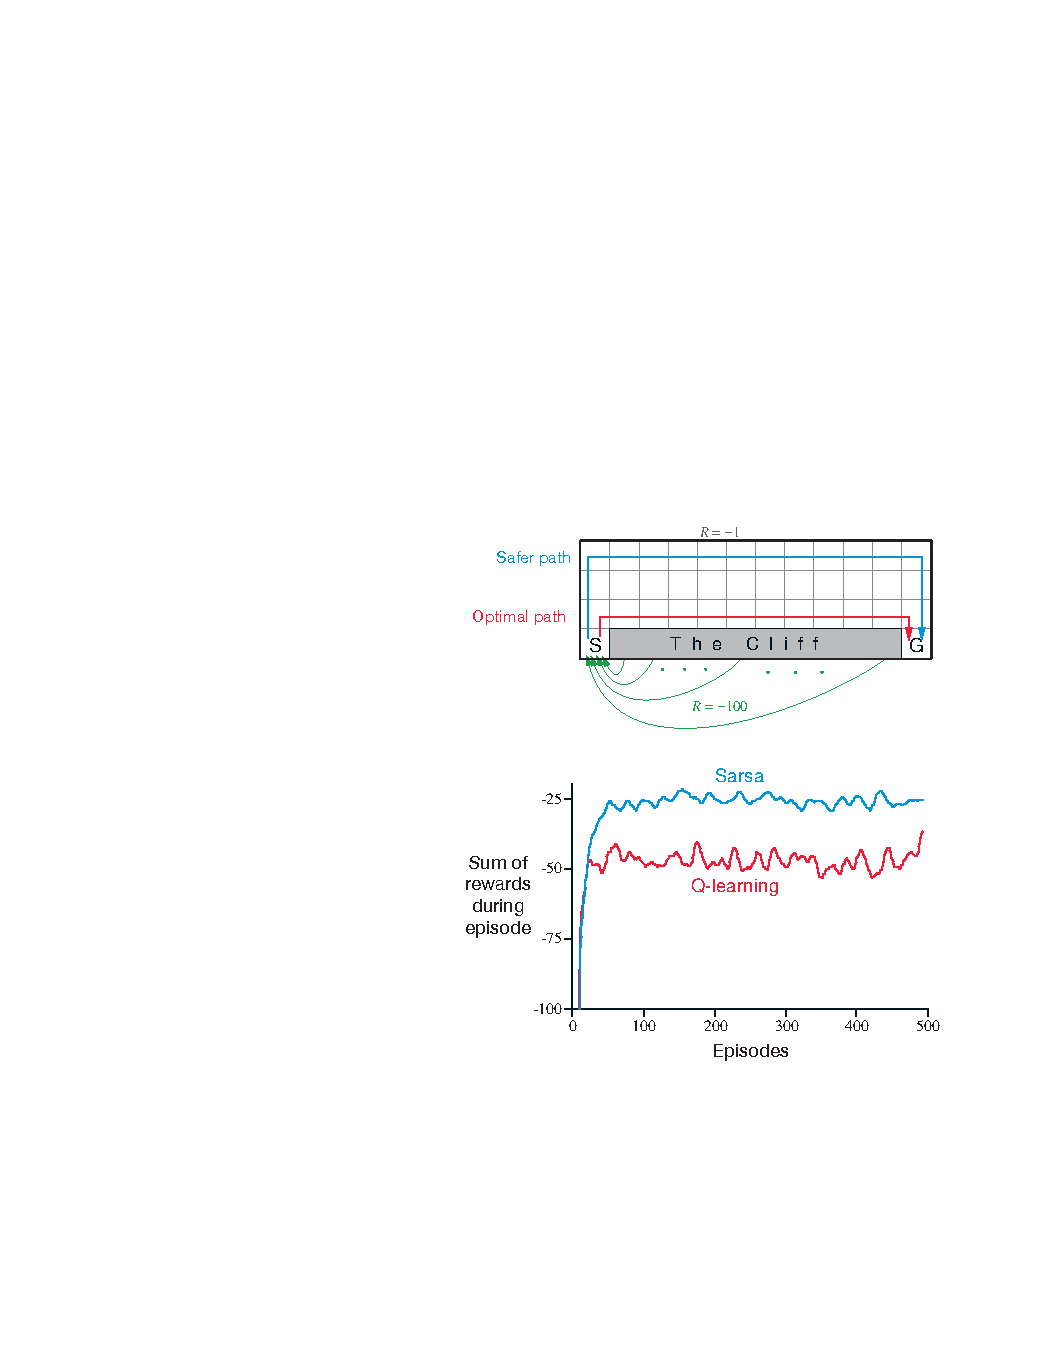
\includegraphics[width=5.5cm]{fig/lec05/Cliff_Walking.pdf}
		\caption{Cliff walking environment (source: R. Sutton and G. Barto, Reinforcement learning: an introduction, 2018, \href{https://creativecommons.org/licenses/by-nc-nd/2.0/}{CC BY-NC-ND 2.0})}
		\label{fig:Cliff_Walking}
	\end{figure}
\end{minipage}
\end{column}
\hfill
\begin{column}{0.40\textwidth}
\begin{minipage}[t]{\linewidth}
	\begin{itemize}
		\item $r=-1$ per time step
		\item Large penalty if you fall off the cliff 
		\item No discounting
		\item $\varepsilon=0.1$
	\end{itemize}
	\vspace{1cm}\pause
	\begin{itemize}
		\item Why is Sarsa better in this example?
		\item And what policy's performance is shown here in particular?
	\end{itemize}
\end{minipage}
\end{column}
\end{columns}
}

%%%%%%%%%%%%%%%%%%%%%%%%%%%%%%%%%%%%%%%%%%%%%%%%%%%%%%%%%%%%%%%%%%
\section{Expected Sarsa} 
%%%%%%%%%%%%%%%%%%%%%%%%%%%%%%%%%%%%%%%%%%%%%%%%%%%%%%%%%%%%%%%%%%
\begin{frame}
\frametitle{Table of Contents}
\tableofcontents[currentsection]
\end{frame}

%%%%%%%%%%%%%%%%%%%%%%%%%%%%%%%%%%%%%%%%%%%%%%%%%%%%%%%%%%%%%
%% Q-Learning Approach %%
%%%%%%%%%%%%%%%%%%%%%%%%%%%%%%%%%%%%%%%%%%%%%%%%%%%%%%%%%%%%%
\frame{\frametitle{Expected Sarsa: A Hybrid Approach}
\begin{block}{Expected Sarsa action-value update}
	The expected Sarsa action-value update is:
		\small
		\begin{equation}
		\begin{split}
		\hat{q}(x_k, u_k) &\leftarrow \hat{q}(x_k, u_k) + \alpha\left[r_{k+1}+\gamma \El{\hat{q}(x_{k+1}, u_{k+1})|x_{k+1}}{\pi} - \hat{q}(x_k, u_k)\right] ,\\
											&\leftarrow \hat{q}(x_k, u_k) + \alpha\left[r_{k+1}+\gamma \sum_{u} \pi(u|x_{k+1}) \hat{q}(x_{k+1}, u) - \hat{q}(x_k, u_k)\right].
		\end{split}
		\label{eq:Expected_Sarsa_update_action_value}
		\end{equation}
		\normalsize
		This is an \hl{off or on-policy} update, depending on whether the action leading to $x_{k+1}$ was taken from the target or a varying behavior policy. 
	\end{block}
\pause
\begin{itemize}
	\item Moves deterministically in the same direction as Sarsa moves in expectation (accordingly, it is called expected Sarsa). \pause
	\item Computationally more complex than Sarsa but reduces variance due to random selection of $u_{k+1}$. \pause
	\item If $\pi$ is greedy and $b$ is an exploratory behavior policy, then expected Sarsa is exactly $Q$-learning (generalization). 
\end{itemize}
}

%%%%%%%%%%%%%%%%%%%%%%%%%%%%%%%%%%%%%%%%%%%%%%%%%%%%%%%%%%%%%
%% Back-up Diagrams for TD-Based Control Approaches %%
%%%%%%%%%%%%%%%%%%%%%%%%%%%%%%%%%%%%%%%%%%%%%%%%%%%%%%%%%%%%%
\frame{\frametitle{Back-up Diagrams for TD-Based Control Approaches}
\begin{minipage}[t]{0.32\linewidth}
	\begin{figure}
		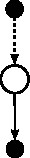
\includegraphics[height=3.0cm]{fig/lec05/Back_Up_Sarsa.pdf}
		\caption{Sarsa}
	\end{figure}
\end{minipage}
\hfill
\begin{minipage}[t]{0.32\linewidth}
	\begin{figure}
		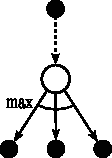
\includegraphics[height=3.0cm]{fig/lec05/Back_Up_Q_learning.pdf}
		\caption{Q-learning}
	\end{figure}
\end{minipage}
\hfill
\begin{minipage}[t]{0.32\linewidth}
	\begin{figure}
		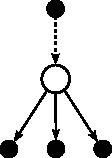
\includegraphics[height=3.0cm]{fig/lec05/Back_Up_Expected_Sarsa.pdf}
		\caption{Expected Sarsa}
	\end{figure}
\end{minipage}
\begin{itemize}
	\item Commonalities:
	\begin{itemize}
		\item Use sample updates based on a one step look ahead evaluation.
		\item Improve estimates based on other estimates (bootstrap). 
	\end{itemize}\pause
	\item Distinctions:
	\begin{itemize}
		\item Sarsa updates based on specific state-action transitions.
		\item $Q$-learning updates the optimal policy estimate $q^*$
		\item Expected Sarsa updates considering the expected transitions.
	\end{itemize}
\end{itemize}
}

%%%%%%%%%%%%%%%%%%%%%%%%%%%%%%%%%%%%%%%%%%%%%%%%%%%%%%%%%%%%%
%% Comparison Based on Cliff-Walking Example %%
%%%%%%%%%%%%%%%%%%%%%%%%%%%%%%%%%%%%%%%%%%%%%%%%%%%%%%%%%%%%%
\frame{\frametitle{Comparison Based on Cliff-Walking Example}
\vspace{-0.2cm}
\begin{figure}		
	\hspace*{-1.0cm}
	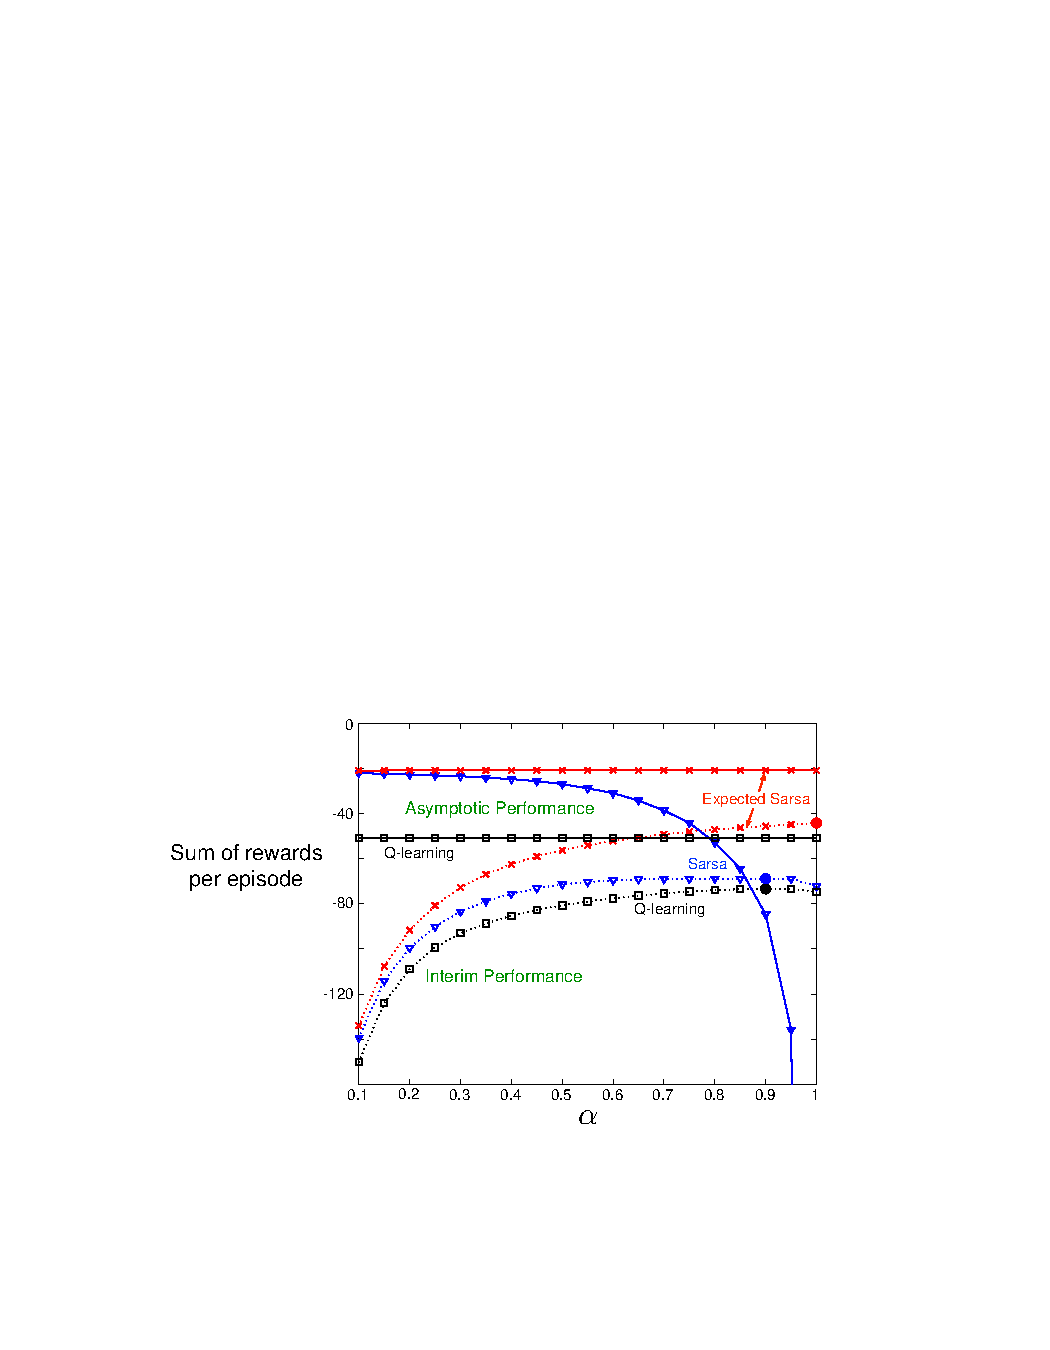
\includegraphics[width=9cm]{fig/lec05/Cliff_Walking_Extended.pdf}
	\caption{All algorithms used an $\varepsilon$-greedy policy with $\varepsilon = 0.1$. Asymptotic performance is an average over 100,000 episodes whereas interim performance is an average over the first 100 episodes. These data are averages of over 50,000 and 10 runs for the interim and asymptotic cases respectively (source: R. Sutton and G. Barto, Reinforcement learning: an introduction, 2018, \href{https://creativecommons.org/licenses/by-nc-nd/2.0/}{CC BY-NC-ND 2.0})}
	\label{Cliff_Walking_Extended}
\end{figure}
}

%%%%%%%%%%%%%%%%%%%%%%%%%%%%%%%%%%%%%%%%%%%%%%%%%%%%%%%%%%%%%%%%%%
\section{Maximization Bias and Double Learning} 
%%%%%%%%%%%%%%%%%%%%%%%%%%%%%%%%%%%%%%%%%%%%%%%%%%%%%%%%%%%%%%%%%%
\begin{frame}
\frametitle{Table of Contents}
\tableofcontents[currentsection]
\end{frame}

%%%%%%%%%%%%%%%%%%%%%%%%%%%%%%%%%%%%%%%%%%%%%%%%%%%%%%%%%%%%%
%% Maximization Bias %%
%%%%%%%%%%%%%%%%%%%%%%%%%%%%%%%%%%%%%%%%%%%%%%%%%%%%%%%%%%%%%
\frame{\frametitle{Maximization Bias}
All control algorithms discussed so far \hl{involve maximization operations}:
\begin{itemize}
	\item $Q$-learning: target policy is greedy and directly uses $\max$ operator for action-value updates.
	\item Sarsa: typically uses an $\varepsilon$-greedy framework, which also involves $\max$ updates during policy improvement.
\end{itemize}\pause
This can lead to a significant \hl{positive bias}:
\begin{itemize}
	\item Maximization over sampled values is used implicitly as an estimate of the maximum value.
	\item This issue is called \hl{maximization bias}.
\end{itemize}\pause
Small example:
\begin{itemize}
	\item Consider a single state $x$ with multiple possible actions $u$.
	\item The true action values are all $q(x,u)=0$ .
	\item The sampled estimates $\hat{q}(x,u)$ are uncertain, i.e., randomly distributed. Some samples are above and below zero.
	\item Consequence: The maximum of the estimate is positive.
\end{itemize}
}

%%%%%%%%%%%%%%%%%%%%%%%%%%%%%%%%%%%%%%%%%%%%%%%%%%%%%%%%%%%%%
%% Double Learning Approach %%
%%%%%%%%%%%%%%%%%%%%%%%%%%%%%%%%%%%%%%%%%%%%%%%%%%%%%%%%%%%%%
\frame{\frametitle{Double Learning Approach}

Split the learning process:
\begin{itemize}
	\item Divide sampled experience into two sets.
	\item Use sets to estimate independent estimates $\hat{q}_1(x,u)$ and $\hat{q}_2(x,u)$.
\end{itemize}\pause
\vspace{0.5cm}
Assign specific tasks to each estimate:
\begin{itemize}
	\item Estimate the maximizing action: 
	\begin{equation}
		 u^*=\argmax_u \hat{q}_1(x,u) .
	\end{equation}\pause
	\item Estimate corresponding action value: 
	\begin{equation}
		q(x,u^*) \approx \hat{q}_2(x,u^*)= \hat{q}_2(x,\argmax_u \hat{q}_1(x,u)) .
	\end{equation}\pause
	\item Doubles memory requirements, but amount of computation per step remains the same.
\end{itemize}
}

%%%%%%%%%%%%%%%%%%%%%%%%%%%%%%%%%%%%%%%%%%%%%%%%%%%%%%%%%%%%%
%% Double Q-Learning Algorithm %%
%%%%%%%%%%%%%%%%%%%%%%%%%%%%%%%%%%%%%%%%%%%%%%%%%%%%%%%%%%%%%
\frame{\frametitle{Double $Q$-Learning Algorithm}
\vspace{0.1cm}
\setlength{\algomargin}{0.5em}
\begin{algorithm}[H]
\footnotesize
\SetKwInput{Input}{input} 
\SetKwInput{Output}{output}
\SetKwInput{Init}{init}
\SetKwInput{Param}{parameter}
\Param{$\varepsilon\in\left\{\mathbb{R}|0<\varepsilon<<1\right\}, \quad \alpha\in\left\{\mathbb{R}|0<\alpha<1\right\}$}
\Init{$\hat{q}_1(x,u),\,\hat{q}_2(x,u)$ arbitrarily (except terminal states) $\forall \, \left\{x\in\mathcal{X}, u\in\mathcal{U}\right\}$}
\For{$j=1,2,\ldots$ episodes}{
	Initialize $x_0$\;
	$k \leftarrow 0$\;
	\Repeat{$x_k$ is terminal}{
				Choose $u_k$ from $x_k$ using the policy $\varepsilon$-greedy based on $\hat{q}_1(x,u)+\hat{q}_2(x,u)$\;
				Take action $u_k$, observe $r_{k+1}$ and $x_{k+1}$\;
				\eIf{$n\sim \mathcal{N}(\mu=0, \sigma)>0$}{
				$\hat{q}_1(x_k, u_k) \leftarrow \hat{q}_1(x_k, u_k) + \alpha\left[r_{k+1}+\gamma \hat{q}_2(x_{k+1}, \argmax_u \hat{q}_1(x_{k+1},u)) - \hat{q}_1(x_k, u_k)\right]$\;}
				{$\hat{q}_2(x_k, u_k) \leftarrow \hat{q}_2(x_k, u_k) + \alpha\left[r_{k+1}+\gamma \hat{q}_1(x_{k+1}, \argmax_u \hat{q}_2(x_{k+1},u)) - \hat{q}_2(x_k, u_k)\right]$\;}
				
				$k \leftarrow k+1$\;
	}
}
\caption{TD-based off-policy control with double learning}
\label{algo:double_Q_learning}
\end{algorithm}
}

%%%%%%%%%%%%%%%%%%%%%%%%%%%%%%%%%%%%%%%%%%%%%%%%%%%%%%%%%%%%%
%% Maximization Bias Example %%
%%%%%%%%%%%%%%%%%%%%%%%%%%%%%%%%%%%%%%%%%%%%%%%%%%%%%%%%%%%%%
\frame{\frametitle{Maximization Bias Example}
\vspace{-0.2cm}
\begin{figure}		
	\hspace*{-1.0cm}
	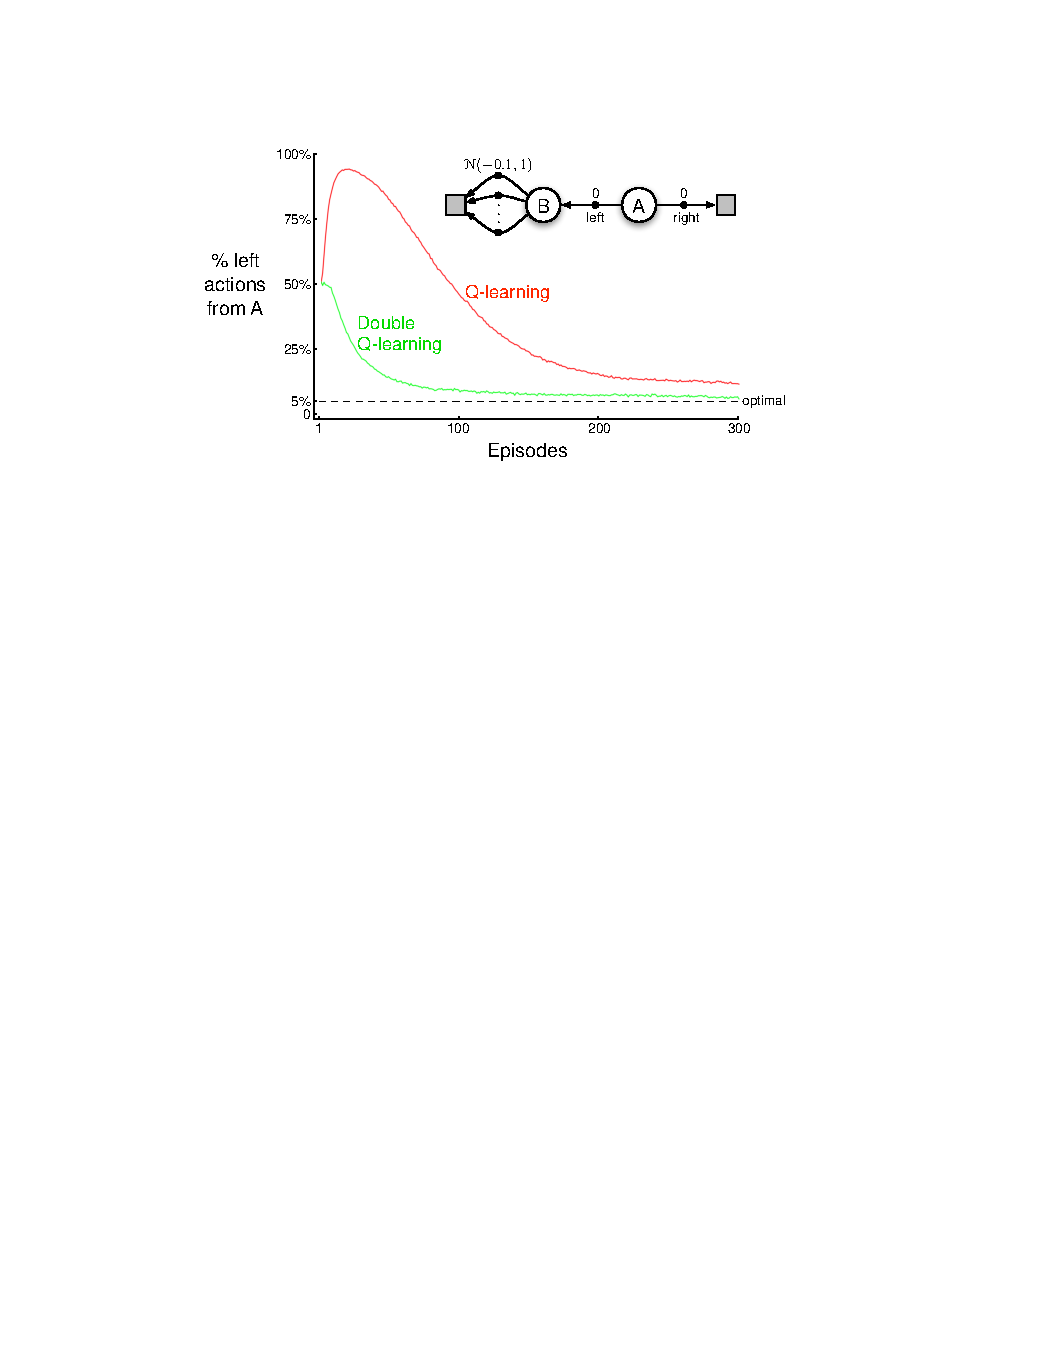
\includegraphics[width=9cm]{fig/lec05/Double_Learning_Example.pdf}
	\caption{Comparison of $Q$-learning and double $Q$-learning on a simple episodic MDP. $Q$-learning initially learns to take the left action much more often than the right action, and always takes it significantly more often than the $5 \%$ minimum probability enforced by $\varepsilon$-greedy action selection with $\varepsilon= 0.1$. In contrast, double $Q$-learning is essentially unaffected by maximization bias. These data are averaged over 10,000 runs. The initial action-value estimates were zero. (source: R. Sutton and G. Barto, Reinforcement learning: an introduction, 2018, \href{https://creativecommons.org/licenses/by-nc-nd/2.0/}{CC BY-NC-ND 2.0})}
	\label{Double_Learning_Example}
\end{figure}
}

%%%%%%%%%%%%%%%%%%%%%%%%%%%%%%%%%%%%%%%%%%%%%%%%%%%%%%%%%%%%%
%% Summary %%
%%%%%%%%%%%%%%%%%%%%%%%%%%%%%%%%%%%%%%%%%%%%%%%%%%%%%%%%%%%%%
\begin{frame}
\frametitle{Summary: What You've Learned Today}
\begin{itemize}
	\item TD unites two key characteristics from DP and MC:
	\begin{itemize}
		\item From MC: Sample-based updates (i.e., operating in unknown MDPs).
		\item From DP: Update estimates based on other estimates (bootstrapping).
	\end{itemize}\pause
	\item TD allows certain simplifications and improvements compared to MC:
	\begin{itemize}
		\item Updates are available after each step and not after each episode.\pause
		\item Off-policy learning comes without importance sampling.\pause
		\item Exploits MDP formalism by maximum likelihood estimates. \pause
		\item Hence, TD prediction and control exhibit a high applicability for many problems.\pause
	\end{itemize}
	\item Batch training can be used when only limited experience is available, i.e., the available samples are re-processed again and again.\pause
	\item Greedy policy improvements can lead to maximization biases and, therefore, slow down the learning process. \pause
	\item TD requires careful tuning of learning parameters:
	\begin{itemize}
		\item Step size $\alpha$: how to tune convergence rate vs. uncertainty / accuracy?
		\item Exploration vs. exploitation: how to visit all state-action pairs?
	\end{itemize}
\end{itemize}
\end{frame}
